\documentclass[1p]{elsarticle_modified}
%\bibliographystyle{elsarticle-num}

%\usepackage[colorlinks]{hyperref}
%\usepackage{abbrmath_seonhwa} %\Abb, \Ascr, \Acal ,\Abf, \Afrak
\usepackage{amsfonts}
\usepackage{amssymb}
\usepackage{amsmath}
\usepackage{amsthm}
\usepackage{scalefnt}
\usepackage{amsbsy}
\usepackage{kotex}
\usepackage{caption}
\usepackage{subfig}
\usepackage{color}
\usepackage{graphicx}
\usepackage{xcolor} %% white, black, red, green, blue, cyan, magenta, yellow
\usepackage{float}
\usepackage{setspace}
\usepackage{hyperref}

\usepackage{tikz}
\usetikzlibrary{arrows}

\usepackage{multirow}
\usepackage{array} % fixed length table
\usepackage{hhline}

%%%%%%%%%%%%%%%%%%%%%
\makeatletter
\renewcommand*\env@matrix[1][\arraystretch]{%
	\edef\arraystretch{#1}%
	\hskip -\arraycolsep
	\let\@ifnextchar\new@ifnextchar
	\array{*\c@MaxMatrixCols c}}
\makeatother %https://tex.stackexchange.com/questions/14071/how-can-i-increase-the-line-spacing-in-a-matrix
%%%%%%%%%%%%%%%

\usepackage[normalem]{ulem}

\newcommand{\msout}[1]{\ifmmode\text{\sout{\ensuremath{#1}}}\else\sout{#1}\fi}
%SOURCE: \msout is \stkout macro in https://tex.stackexchange.com/questions/20609/strikeout-in-math-mode

\newcommand{\cancel}[1]{
	\ifmmode
	{\color{red}\msout{#1}}
	\else
	{\color{red}\sout{#1}}
	\fi
}

\newcommand{\add}[1]{
	{\color{blue}\uwave{#1}}
}

\newcommand{\replace}[2]{
	\ifmmode
	{\color{red}\msout{#1}}{\color{blue}\uwave{#2}}
	\else
	{\color{red}\sout{#1}}{\color{blue}\uwave{#2}}
	\fi
}

\newcommand{\Sol}{\mathcal{S}} %segment
\newcommand{\D}{D} %diagram
\newcommand{\A}{\mathcal{A}} %arc


%%%%%%%%%%%%%%%%%%%%%%%%%%%%%5 test

\def\sl{\operatorname{\textup{SL}}(2,\Cbb)}
\def\psl{\operatorname{\textup{PSL}}(2,\Cbb)}
\def\quan{\mkern 1mu \triangleright \mkern 1mu}

\theoremstyle{definition}
\newtheorem{thm}{Theorem}[section]
\newtheorem{prop}[thm]{Proposition}
\newtheorem{lem}[thm]{Lemma}
\newtheorem{ques}[thm]{Question}
\newtheorem{cor}[thm]{Corollary}
\newtheorem{defn}[thm]{Definition}
\newtheorem{exam}[thm]{Example}
\newtheorem{rmk}[thm]{Remark}
\newtheorem{alg}[thm]{Algorithm}

\newcommand{\I}{\sqrt{-1}}
\begin{document}

%\begin{frontmatter}
%
%\title{Boundary parabolic representations of knots up to 8 crossings}
%
%%% Group authors per affiliation:
%\author{Yunhi Cho} 
%\address{Department of Mathematics, University of Seoul, Seoul, Korea}
%\ead{yhcho@uos.ac.kr}
%
%
%\author{Seonhwa Kim} %\fnref{s_kim}}
%\address{Center for Geometry and Physics, Institute for Basic Science, Pohang, 37673, Korea}
%\ead{ryeona17@ibs.re.kr}
%
%\author{Hyuk Kim}
%\address{Department of Mathematical Sciences, Seoul National University, Seoul 08826, Korea}
%\ead{hyukkim@snu.ac.kr}
%
%\author{Seokbeom Yoon}
%\address{Department of Mathematical Sciences, Seoul National University, Seoul, 08826,  Korea}
%\ead{sbyoon15@snu.ac.kr}
%
%\begin{abstract}
%We find all boundary parabolic representation of knots up to 8 crossings.
%
%\end{abstract}
%\begin{keyword}
%    \MSC[2010] 57M25 
%\end{keyword}
%
%\end{frontmatter}

%\linenumbers
%\tableofcontents
%
\newcommand\colored[1]{\textcolor{white}{\rule[-0.35ex]{0.8em}{1.4ex}}\kern-0.8em\color{red} #1}%
%\newcommand\colored[1]{\textcolor{white}{ #1}\kern-2.17ex	\textcolor{white}{ #1}\kern-1.81ex	\textcolor{white}{ #1}\kern-2.15ex\color{red}#1	}

{\Large $\underline{12a_{0964}~(K12a_{0964})}$}

\setlength{\tabcolsep}{10pt}
\renewcommand{\arraystretch}{1.6}
\vspace{1cm}\begin{tabular}{m{100pt}>{\centering\arraybackslash}m{274pt}}
\multirow{5}{120pt}{
	\centering
	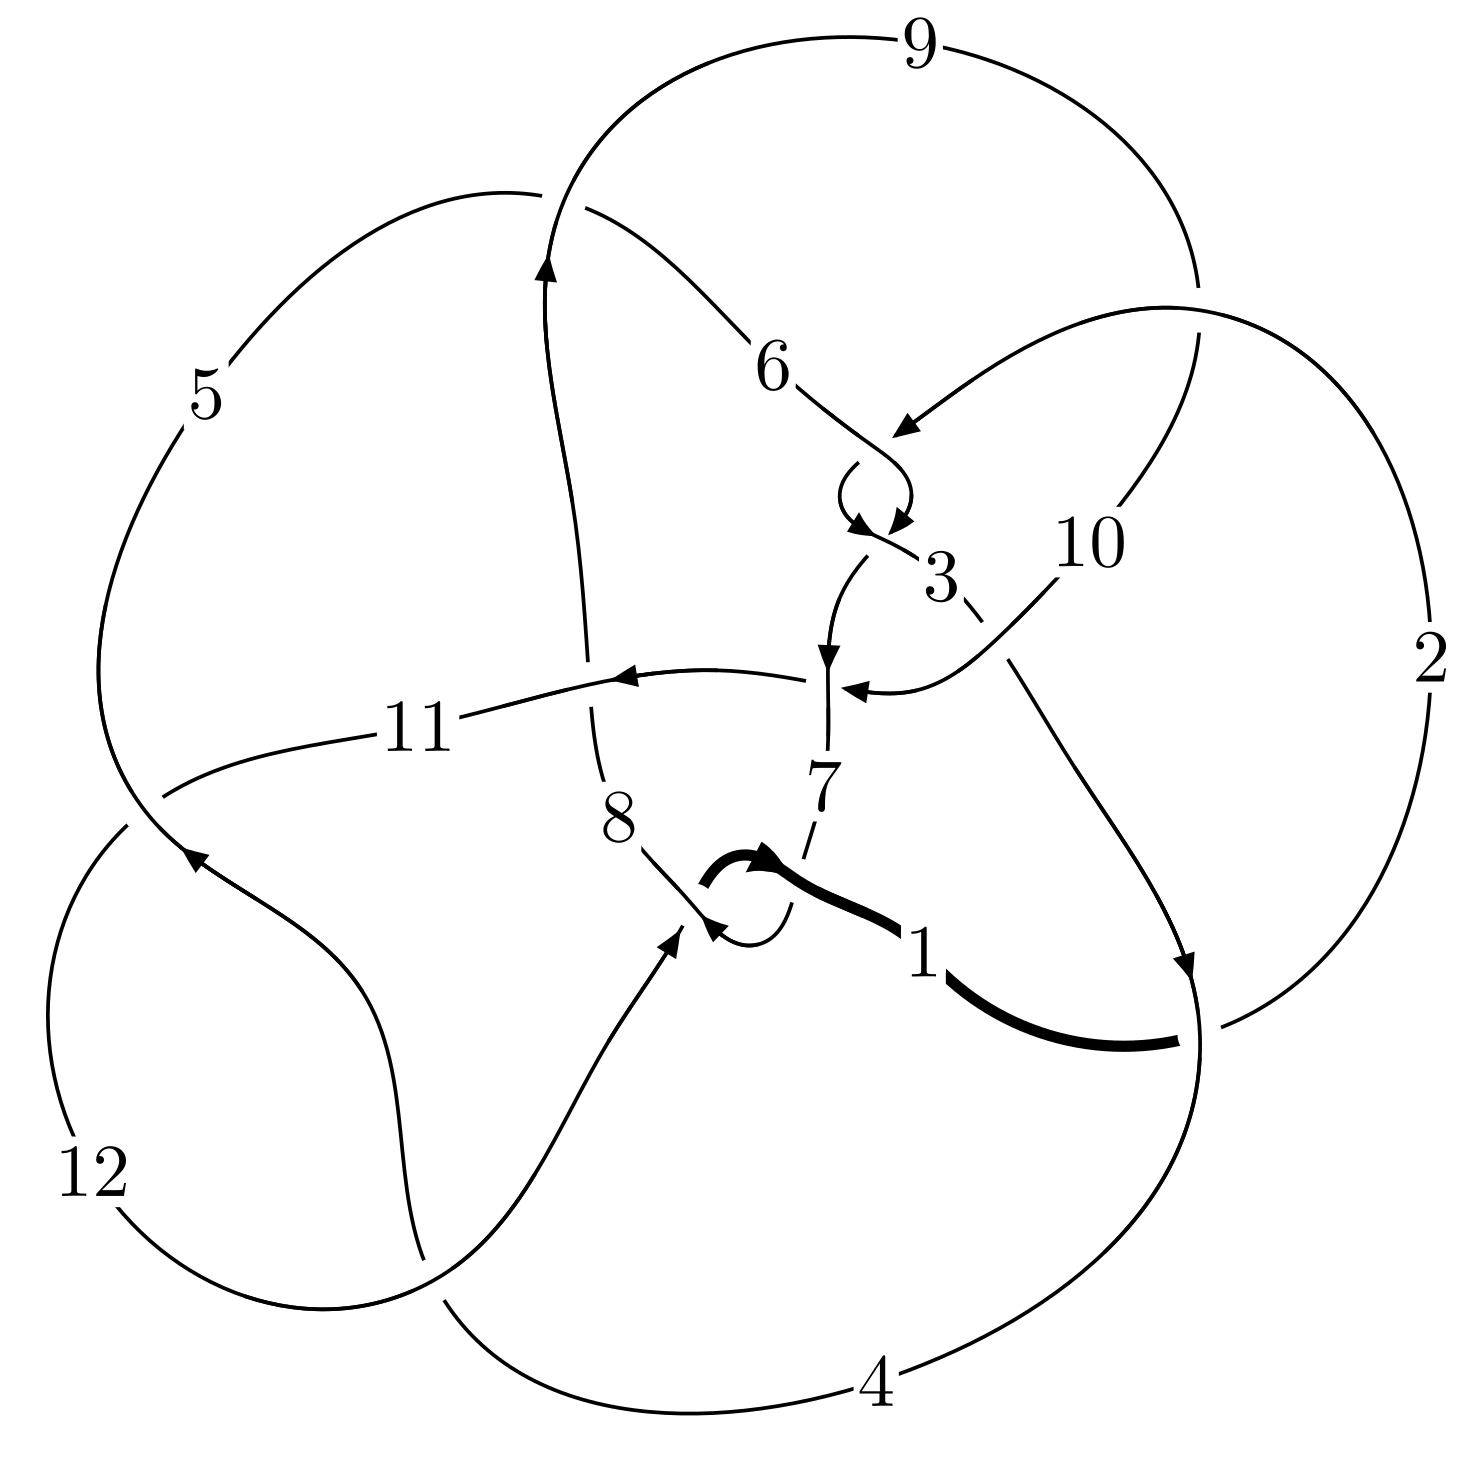
\includegraphics[width=112pt]{../../../GIT/diagram.site/Diagrams/png/1765_12a_0964.png}\\
\ \ \ A knot diagram\footnotemark}&
\allowdisplaybreaks
\textbf{Linearized knot diagam} \\
\cline{2-2}
 &
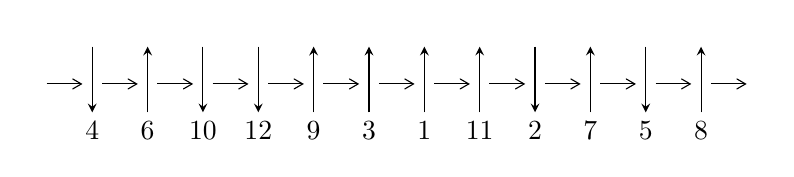
\begin{tikzpicture}[x=20pt, y=17pt]
	% nodes
	\node (C0) at (0, 0) {};
	\node (C1) at (1, 0) {};
	\node (C1U) at (1, +1) {};
	\node (C1D) at (1, -1) {4};

	\node (C2) at (2, 0) {};
	\node (C2U) at (2, +1) {};
	\node (C2D) at (2, -1) {6};

	\node (C3) at (3, 0) {};
	\node (C3U) at (3, +1) {};
	\node (C3D) at (3, -1) {10};

	\node (C4) at (4, 0) {};
	\node (C4U) at (4, +1) {};
	\node (C4D) at (4, -1) {12};

	\node (C5) at (5, 0) {};
	\node (C5U) at (5, +1) {};
	\node (C5D) at (5, -1) {9};

	\node (C6) at (6, 0) {};
	\node (C6U) at (6, +1) {};
	\node (C6D) at (6, -1) {3};

	\node (C7) at (7, 0) {};
	\node (C7U) at (7, +1) {};
	\node (C7D) at (7, -1) {1};

	\node (C8) at (8, 0) {};
	\node (C8U) at (8, +1) {};
	\node (C8D) at (8, -1) {11};

	\node (C9) at (9, 0) {};
	\node (C9U) at (9, +1) {};
	\node (C9D) at (9, -1) {2};

	\node (C10) at (10, 0) {};
	\node (C10U) at (10, +1) {};
	\node (C10D) at (10, -1) {7};

	\node (C11) at (11, 0) {};
	\node (C11U) at (11, +1) {};
	\node (C11D) at (11, -1) {5};

	\node (C12) at (12, 0) {};
	\node (C12U) at (12, +1) {};
	\node (C12D) at (12, -1) {8};
	\node (C13) at (13, 0) {};

	% arrows
	\draw[->,>={angle 60}]
	(C0) edge (C1) (C1) edge (C2) (C2) edge (C3) (C3) edge (C4) (C4) edge (C5) (C5) edge (C6) (C6) edge (C7) (C7) edge (C8) (C8) edge (C9) (C9) edge (C10) (C10) edge (C11) (C11) edge (C12) (C12) edge (C13) ;	\draw[->,>=stealth]
	(C1U) edge (C1D) (C2D) edge (C2U) (C3U) edge (C3D) (C4U) edge (C4D) (C5D) edge (C5U) (C6D) edge (C6U) (C7D) edge (C7U) (C8D) edge (C8U) (C9U) edge (C9D) (C10D) edge (C10U) (C11U) edge (C11D) (C12D) edge (C12U) ;
	\end{tikzpicture} \\
\hhline{~~} \\& 
\textbf{Solving Sequence} \\ \cline{2-2} 
 &
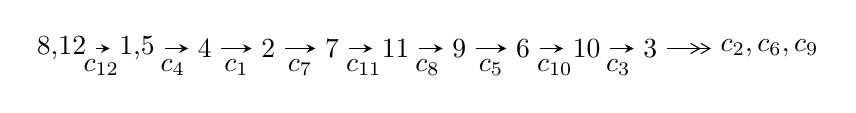
\begin{tikzpicture}[x=23pt, y=7pt]
	% node
	\node (A0) at (-1/8, 0) {8,12};
	\node (A1) at (17/16, 0) {1,5};
	\node (A2) at (17/8, 0) {4};
	\node (A3) at (25/8, 0) {2};
	\node (A4) at (33/8, 0) {7};
	\node (A5) at (41/8, 0) {11};
	\node (A6) at (49/8, 0) {9};
	\node (A7) at (57/8, 0) {6};
	\node (A8) at (65/8, 0) {10};
	\node (A9) at (73/8, 0) {3};
	\node (C1) at (1/2, -1) {$c_{12}$};
	\node (C2) at (13/8, -1) {$c_{4}$};
	\node (C3) at (21/8, -1) {$c_{1}$};
	\node (C4) at (29/8, -1) {$c_{7}$};
	\node (C5) at (37/8, -1) {$c_{11}$};
	\node (C6) at (45/8, -1) {$c_{8}$};
	\node (C7) at (53/8, -1) {$c_{5}$};
	\node (C8) at (61/8, -1) {$c_{10}$};
	\node (C9) at (69/8, -1) {$c_{3}$};
	\node (A10) at (11, 0) {$c_{2},c_{6},c_{9}$};

	% edge
	\draw[->,>=stealth]	
	(A0) edge (A1) (A1) edge (A2) (A2) edge (A3) (A3) edge (A4) (A4) edge (A5) (A5) edge (A6) (A6) edge (A7) (A7) edge (A8) (A8) edge (A9) ;
	\draw[->>,>={angle 60}]	
	(A9) edge (A10);
\end{tikzpicture} \\ 

\end{tabular} \\

\footnotetext{
The image of knot diagram is generated by the software ``\textbf{Draw programme}" developed by Andrew Bartholomew(\url{http://www.layer8.co.uk/maths/draw/index.htm\#Running-draw}), where we modified some parts for our purpose(\url{https://github.com/CATsTAILs/LinksPainter}).
}\phantom \\ \newline 
\centering \textbf{Ideals for irreducible components\footnotemark of $X_{\text{par}}$} 
 
\begin{align*}
I^u_{1}&=\langle 
-6.67140\times10^{1041} u^{172}+3.09638\times10^{1041} u^{171}+\cdots+4.13995\times10^{1042} b-2.35617\times10^{1044},\\
\phantom{I^u_{1}}&\phantom{= \langle  }-1.43628\times10^{1045} u^{172}+4.80688\times10^{1045} u^{171}+\cdots+1.05606\times10^{1047} a-1.79297\times10^{1049},\\
\phantom{I^u_{1}}&\phantom{= \langle  }u^{173}+56 u^{171}+\cdots+10670 u-773\rangle \\
I^u_{2}&=\langle 
1.19997\times10^{42} u^{45}+2.62403\times10^{42} u^{44}+\cdots+5.23068\times10^{41} b+2.29859\times10^{42},\\
\phantom{I^u_{2}}&\phantom{= \langle  }-1.94564\times10^{42} u^{45}-3.70634\times10^{42} u^{44}+\cdots+5.23068\times10^{41} a-4.20375\times10^{42},\;u^{46}+u^{45}+\cdots+7 u^2+1\rangle \\
\\
\end{align*}
\raggedright * 2 irreducible components of $\dim_{\mathbb{C}}=0$, with total 219 representations.\\
\footnotetext{All coefficients of polynomials are rational numbers. But the coefficients are sometimes approximated in decimal forms when there is not enough margin.}
\newpage
\renewcommand{\arraystretch}{1}
\centering \section*{I. $I^u_{1}= \langle -6.67\times10^{1041} u^{172}+3.10\times10^{1041} u^{171}+\cdots+4.14\times10^{1042} b-2.36\times10^{1044},\;-1.44\times10^{1045} u^{172}+4.81\times10^{1045} u^{171}+\cdots+1.06\times10^{1047} a-1.79\times10^{1049},\;u^{173}+56 u^{171}+\cdots+10670 u-773 \rangle$}
\flushleft \textbf{(i) Arc colorings}\\
\begin{tabular}{m{7pt} m{180pt} m{7pt} m{180pt} }
\flushright $a_{8}=$&$\begin{pmatrix}0\\u\end{pmatrix}$ \\
\flushright $a_{12}=$&$\begin{pmatrix}1\\0\end{pmatrix}$ \\
\flushright $a_{1}=$&$\begin{pmatrix}1\\- u^2\end{pmatrix}$ \\
\flushright $a_{5}=$&$\begin{pmatrix}0.0136004 u^{172}-0.0455171 u^{171}+\cdots-2485.94 u+169.780\\0.161147 u^{172}-0.0747927 u^{171}+\cdots-1077.27 u+56.9130\end{pmatrix}$ \\
\flushright $a_{4}=$&$\begin{pmatrix}0.174747 u^{172}-0.120310 u^{171}+\cdots-3563.20 u+226.693\\0.161147 u^{172}-0.0747927 u^{171}+\cdots-1077.27 u+56.9130\end{pmatrix}$ \\
\flushright $a_{2}=$&$\begin{pmatrix}-0.303815 u^{172}+0.326187 u^{171}+\cdots+6959.17 u-467.508\\0.0438291 u^{172}-0.100993 u^{171}+\cdots-1973.22 u+136.971\end{pmatrix}$ \\
\flushright $a_{7}=$&$\begin{pmatrix}- u\\u^3+u\end{pmatrix}$ \\
\flushright $a_{11}=$&$\begin{pmatrix}0.116379 u^{172}-0.217688 u^{171}+\cdots-4690.20 u+326.071\\0.0203251 u^{172}-0.0330088 u^{171}+\cdots-807.396 u+56.8178\end{pmatrix}$ \\
\flushright $a_{9}=$&$\begin{pmatrix}0.198840 u^{172}+0.227474 u^{171}+\cdots+4526.36 u-349.016\\-0.0976959 u^{172}-0.0685834 u^{171}+\cdots-1497.85 u+119.447\end{pmatrix}$ \\
\flushright $a_{6}=$&$\begin{pmatrix}-0.0838203 u^{172}+0.122068 u^{171}+\cdots+2178.16 u-151.864\\-0.000493639 u^{172}-0.0509278 u^{171}+\cdots-751.488 u+53.5767\end{pmatrix}$ \\
\flushright $a_{10}=$&$\begin{pmatrix}0.160851 u^{172}-0.290478 u^{171}+\cdots-6214.35 u+431.481\\-0.00126672 u^{172}-0.00132586 u^{171}+\cdots-94.2923 u+7.67446\end{pmatrix}$ \\
\flushright $a_{3}=$&$\begin{pmatrix}-0.178003 u^{172}-0.100257 u^{171}+\cdots-2553.46 u+209.740\\0.119152 u^{172}-0.0509618 u^{171}+\cdots-1079.46 u+60.1908\end{pmatrix}$\\&\end{tabular}
\flushleft \textbf{(ii) Obstruction class $= -1$}\\~\\
\flushleft \textbf{(iii) Cusp Shapes $= 0.859602 u^{172}-0.0626764 u^{171}+\cdots+1294.31 u-186.370$}\\~\\
\newpage\renewcommand{\arraystretch}{1}
\flushleft \textbf{(iv) u-Polynomials at the component}\newline \\
\begin{tabular}{m{50pt}|m{274pt}}
Crossings & \hspace{64pt}u-Polynomials at each crossing \\
\hline $$\begin{aligned}c_{1}\end{aligned}$$&$\begin{aligned}
&u^{173}-16 u^{172}+\cdots-441583301 u+43116743
\end{aligned}$\\
\hline $$\begin{aligned}c_{2},c_{6}\end{aligned}$$&$\begin{aligned}
&u^{173}-60 u^{171}+\cdots+941 u-46
\end{aligned}$\\
\hline $$\begin{aligned}c_{3}\end{aligned}$$&$\begin{aligned}
&u^{173}+u^{172}+\cdots-3987176 u+407744
\end{aligned}$\\
\hline $$\begin{aligned}c_{4},c_{11}\end{aligned}$$&$\begin{aligned}
&u^{173}+2 u^{172}+\cdots-87232 u+26609
\end{aligned}$\\
\hline $$\begin{aligned}c_{5}\end{aligned}$$&$\begin{aligned}
&u^{173}-5 u^{172}+\cdots-8202271939895 u+2872546990775
\end{aligned}$\\
\hline $$\begin{aligned}c_{7},c_{12}\end{aligned}$$&$\begin{aligned}
&u^{173}+56 u^{171}+\cdots+10670 u-773
\end{aligned}$\\
\hline $$\begin{aligned}c_{8}\end{aligned}$$&$\begin{aligned}
&u^{173}-7 u^{172}+\cdots-233712855 u-195784578
\end{aligned}$\\
\hline $$\begin{aligned}c_{9}\end{aligned}$$&$\begin{aligned}
&u^{173}-3 u^{172}+\cdots-31113171 u+17614861
\end{aligned}$\\
\hline $$\begin{aligned}c_{10}\end{aligned}$$&$\begin{aligned}
&u^{173}+u^{172}+\cdots-7778112 u-1549121
\end{aligned}$\\
\hline
\end{tabular}\\~\\
\newpage\renewcommand{\arraystretch}{1}
\flushleft \textbf{(v) Riley Polynomials at the component}\newline \\
\begin{tabular}{m{50pt}|m{274pt}}
Crossings & \hspace{64pt}Riley Polynomials at each crossing \\
\hline $$\begin{aligned}c_{1}\end{aligned}$$&$\begin{aligned}
&y^{173}+46 y^{172}+\cdots-190330317939755079 y-1859053526928049
\end{aligned}$\\
\hline $$\begin{aligned}c_{2},c_{6}\end{aligned}$$&$\begin{aligned}
&y^{173}-120 y^{172}+\cdots+29145 y-2116
\end{aligned}$\\
\hline $$\begin{aligned}c_{3}\end{aligned}$$&$\begin{aligned}
&y^{173}+37 y^{172}+\cdots-6492833858112 y-166255169536
\end{aligned}$\\
\hline $$\begin{aligned}c_{4},c_{11}\end{aligned}$$&$\begin{aligned}
&y^{173}+108 y^{172}+\cdots-22481206172 y-708038881
\end{aligned}$\\
\hline $$\begin{aligned}c_{5}\end{aligned}$$&$\begin{aligned}
&y^{173}-117 y^{172}+\cdots+4.33\times10^{26} y-8.25\times10^{24}
\end{aligned}$\\
\hline $$\begin{aligned}c_{7},c_{12}\end{aligned}$$&$\begin{aligned}
&y^{173}+112 y^{172}+\cdots-5655354 y-597529
\end{aligned}$\\
\hline $$\begin{aligned}c_{8}\end{aligned}$$&$\begin{aligned}
&y^{173}-49 y^{172}+\cdots-114284276837571771 y-38331600982638084
\end{aligned}$\\
\hline $$\begin{aligned}c_{9}\end{aligned}$$&$\begin{aligned}
&y^{173}+75 y^{172}+\cdots-248969562329698517 y-310283328049321
\end{aligned}$\\
\hline $$\begin{aligned}c_{10}\end{aligned}$$&$\begin{aligned}
&y^{173}-59 y^{172}+\cdots+217933860538318 y-2399775872641
\end{aligned}$\\
\hline
\end{tabular}\\~\\
\newpage\flushleft \textbf{(vi) Complex Volumes and Cusp Shapes}
$$\begin{array}{c|c|c}  
\text{Solutions to }I^u_{1}& \I (\text{vol} + \sqrt{-1}CS) & \text{Cusp shape}\\
 \hline 
\begin{aligned}
u &= -0.101122 + 1.000200 I \\
a &= \phantom{-}0.799044 - 0.091903 I \\
b &= -0.228446 + 0.904398 I\end{aligned}
 & \phantom{-}3.20434 + 4.19259 I & \phantom{-0.000000 } 0 \\ \hline\begin{aligned}
u &= -0.101122 - 1.000200 I \\
a &= \phantom{-}0.799044 + 0.091903 I \\
b &= -0.228446 - 0.904398 I\end{aligned}
 & \phantom{-}3.20434 - 4.19259 I & \phantom{-0.000000 } 0 \\ \hline\begin{aligned}
u &= \phantom{-}0.479693 + 0.887297 I \\
a &= \phantom{-}0.583507 - 0.266915 I \\
b &= -0.171458 + 0.210995 I\end{aligned}
 & \phantom{-}2.96684 + 3.72671 I & \phantom{-0.000000 } 0 \\ \hline\begin{aligned}
u &= \phantom{-}0.479693 - 0.887297 I \\
a &= \phantom{-}0.583507 + 0.266915 I \\
b &= -0.171458 - 0.210995 I\end{aligned}
 & \phantom{-}2.96684 - 3.72671 I & \phantom{-0.000000 } 0 \\ \hline\begin{aligned}
u &= \phantom{-}0.684518 + 0.716218 I \\
a &= -1.15411 - 1.22058 I \\
b &= -0.677062 + 1.199530 I\end{aligned}
 & \phantom{-}8.65635 + 8.35807 I & \phantom{-0.000000 } 0 \\ \hline\begin{aligned}
u &= \phantom{-}0.684518 - 0.716218 I \\
a &= -1.15411 + 1.22058 I \\
b &= -0.677062 - 1.199530 I\end{aligned}
 & \phantom{-}8.65635 - 8.35807 I & \phantom{-0.000000 } 0 \\ \hline\begin{aligned}
u &= -0.245321 + 0.983911 I \\
a &= \phantom{-}0.103909 + 0.558063 I \\
b &= \phantom{-}0.551768 - 0.219856 I\end{aligned}
 & -1.04505 + 1.01441 I & \phantom{-0.000000 } 0 \\ \hline\begin{aligned}
u &= -0.245321 - 0.983911 I \\
a &= \phantom{-}0.103909 - 0.558063 I \\
b &= \phantom{-}0.551768 + 0.219856 I\end{aligned}
 & -1.04505 - 1.01441 I & \phantom{-0.000000 } 0 \\ \hline\begin{aligned}
u &= \phantom{-}0.247804 + 0.991903 I \\
a &= \phantom{-}0.313803 + 0.200311 I \\
b &= \phantom{-}1.58087 + 0.00415 I\end{aligned}
 & -2.15969 + 3.22516 I & \phantom{-0.000000 } 0 \\ \hline\begin{aligned}
u &= \phantom{-}0.247804 - 0.991903 I \\
a &= \phantom{-}0.313803 - 0.200311 I \\
b &= \phantom{-}1.58087 - 0.00415 I\end{aligned}
 & -2.15969 - 3.22516 I & \phantom{-0.000000 } 0\\
 \hline 
 \end{array}$$\newpage$$\begin{array}{c|c|c}  
\text{Solutions to }I^u_{1}& \I (\text{vol} + \sqrt{-1}CS) & \text{Cusp shape}\\
 \hline 
\begin{aligned}
u &= -0.452563 + 0.860241 I \\
a &= \phantom{-}1.81653 - 0.89243 I \\
b &= \phantom{-}0.026665 + 1.016820 I\end{aligned}
 & \phantom{-}3.37257 + 0.03215 I & \phantom{-0.000000 } 0 \\ \hline\begin{aligned}
u &= -0.452563 - 0.860241 I \\
a &= \phantom{-}1.81653 + 0.89243 I \\
b &= \phantom{-}0.026665 - 1.016820 I\end{aligned}
 & \phantom{-}3.37257 - 0.03215 I & \phantom{-0.000000 } 0 \\ \hline\begin{aligned}
u &= \phantom{-}0.502702 + 0.827109 I \\
a &= -1.26440 - 0.65185 I \\
b &= -0.72703 + 1.28142 I\end{aligned}
 & \phantom{-}9.13038 - 3.72909 I & \phantom{-0.000000 } 0 \\ \hline\begin{aligned}
u &= \phantom{-}0.502702 - 0.827109 I \\
a &= -1.26440 + 0.65185 I \\
b &= -0.72703 - 1.28142 I\end{aligned}
 & \phantom{-}9.13038 + 3.72909 I & \phantom{-0.000000 } 0 \\ \hline\begin{aligned}
u &= \phantom{-}1.051260 + 0.070820 I \\
a &= \phantom{-}0.197185 + 0.953230 I \\
b &= -0.140570 - 0.989697 I\end{aligned}
 & \phantom{-}4.80380 + 0.08961 I & \phantom{-0.000000 } 0 \\ \hline\begin{aligned}
u &= \phantom{-}1.051260 - 0.070820 I \\
a &= \phantom{-}0.197185 - 0.953230 I \\
b &= -0.140570 + 0.989697 I\end{aligned}
 & \phantom{-}4.80380 - 0.08961 I & \phantom{-0.000000 } 0 \\ \hline\begin{aligned}
u &= -0.888495 + 0.570057 I \\
a &= -0.68977 + 1.31626 I \\
b &= \phantom{-}0.457178 - 1.307230 I\end{aligned}
 & \phantom{-}8.48181 + 4.86174 I & \phantom{-0.000000 } 0 \\ \hline\begin{aligned}
u &= -0.888495 - 0.570057 I \\
a &= -0.68977 - 1.31626 I \\
b &= \phantom{-}0.457178 + 1.307230 I\end{aligned}
 & \phantom{-}8.48181 - 4.86174 I & \phantom{-0.000000 } 0 \\ \hline\begin{aligned}
u &= \phantom{-}0.623691 + 0.862271 I \\
a &= \phantom{-}1.064140 + 0.882356 I \\
b &= \phantom{-}0.67592 - 1.27062 I\end{aligned}
 & \phantom{-}4.37248 + 2.06970 I & \phantom{-0.000000 } 0 \\ \hline\begin{aligned}
u &= \phantom{-}0.623691 - 0.862271 I \\
a &= \phantom{-}1.064140 - 0.882356 I \\
b &= \phantom{-}0.67592 + 1.27062 I\end{aligned}
 & \phantom{-}4.37248 - 2.06970 I & \phantom{-0.000000 } 0\\
 \hline 
 \end{array}$$\newpage$$\begin{array}{c|c|c}  
\text{Solutions to }I^u_{1}& \I (\text{vol} + \sqrt{-1}CS) & \text{Cusp shape}\\
 \hline 
\begin{aligned}
u &= \phantom{-}0.478697 + 0.966168 I \\
a &= \phantom{-}0.031951 - 0.456162 I \\
b &= -1.216790 - 0.228920 I\end{aligned}
 & \phantom{-}3.08104 + 4.01412 I & \phantom{-0.000000 } 0 \\ \hline\begin{aligned}
u &= \phantom{-}0.478697 - 0.966168 I \\
a &= \phantom{-}0.031951 + 0.456162 I \\
b &= -1.216790 + 0.228920 I\end{aligned}
 & \phantom{-}3.08104 - 4.01412 I & \phantom{-0.000000 } 0 \\ \hline\begin{aligned}
u &= \phantom{-}0.194997 + 0.899230 I \\
a &= -0.544039 - 0.139825 I \\
b &= -1.65280 - 0.59175 I\end{aligned}
 & -1.73084 - 1.38533 I & \phantom{-0.000000 } 0 \\ \hline\begin{aligned}
u &= \phantom{-}0.194997 - 0.899230 I \\
a &= -0.544039 + 0.139825 I \\
b &= -1.65280 + 0.59175 I\end{aligned}
 & -1.73084 + 1.38533 I & \phantom{-0.000000 } 0 \\ \hline\begin{aligned}
u &= -0.357024 + 0.842769 I \\
a &= -2.10462 + 0.48586 I \\
b &= -0.072531 - 1.177410 I\end{aligned}
 & \phantom{-}7.64728 + 0.79131 I & \phantom{-0.000000 } 0 \\ \hline\begin{aligned}
u &= -0.357024 - 0.842769 I \\
a &= -2.10462 - 0.48586 I \\
b &= -0.072531 + 1.177410 I\end{aligned}
 & \phantom{-}7.64728 - 0.79131 I & \phantom{-0.000000 } 0 \\ \hline\begin{aligned}
u &= -0.442178 + 0.998072 I \\
a &= \phantom{-}1.54070 - 0.80320 I \\
b &= \phantom{-}0.547817 + 1.276240 I\end{aligned}
 & \phantom{-}7.81986 - 5.31031 I & \phantom{-0.000000 } 0 \\ \hline\begin{aligned}
u &= -0.442178 - 0.998072 I \\
a &= \phantom{-}1.54070 + 0.80320 I \\
b &= \phantom{-}0.547817 - 1.276240 I\end{aligned}
 & \phantom{-}7.81986 + 5.31031 I & \phantom{-0.000000 } 0 \\ \hline\begin{aligned}
u &= -0.269968 + 1.060710 I \\
a &= -0.879519 - 0.323573 I \\
b &= -0.815784 - 0.628932 I\end{aligned}
 & \phantom{-}0.08698 - 4.07177 I & \phantom{-0.000000 } 0 \\ \hline\begin{aligned}
u &= -0.269968 - 1.060710 I \\
a &= -0.879519 + 0.323573 I \\
b &= -0.815784 + 0.628932 I\end{aligned}
 & \phantom{-}0.08698 + 4.07177 I & \phantom{-0.000000 } 0\\
 \hline 
 \end{array}$$\newpage$$\begin{array}{c|c|c}  
\text{Solutions to }I^u_{1}& \I (\text{vol} + \sqrt{-1}CS) & \text{Cusp shape}\\
 \hline 
\begin{aligned}
u &= \phantom{-}0.314739 + 1.056770 I \\
a &= \phantom{-}2.52866 - 0.26316 I \\
b &= \phantom{-}0.073179 - 1.081650 I\end{aligned}
 & \phantom{-}7.22069 + 8.60281 I & \phantom{-0.000000 } 0 \\ \hline\begin{aligned}
u &= \phantom{-}0.314739 - 1.056770 I \\
a &= \phantom{-}2.52866 + 0.26316 I \\
b &= \phantom{-}0.073179 + 1.081650 I\end{aligned}
 & \phantom{-}7.22069 - 8.60281 I & \phantom{-0.000000 } 0 \\ \hline\begin{aligned}
u &= -0.833603 + 0.326148 I \\
a &= \phantom{-}0.42708 + 1.96386 I \\
b &= -0.244492 - 1.351940 I\end{aligned}
 & \phantom{-}7.79715 - 5.79779 I & \phantom{-0.000000 } 0 \\ \hline\begin{aligned}
u &= -0.833603 - 0.326148 I \\
a &= \phantom{-}0.42708 - 1.96386 I \\
b &= -0.244492 + 1.351940 I\end{aligned}
 & \phantom{-}7.79715 + 5.79779 I & \phantom{-0.000000 } 0 \\ \hline\begin{aligned}
u &= -0.301341 + 0.840893 I \\
a &= -0.53830 + 1.99359 I \\
b &= -0.06151 - 1.49244 I\end{aligned}
 & \phantom{-}7.75387 - 3.72131 I & \phantom{-0.000000 } 0 \\ \hline\begin{aligned}
u &= -0.301341 - 0.840893 I \\
a &= -0.53830 - 1.99359 I \\
b &= -0.06151 + 1.49244 I\end{aligned}
 & \phantom{-}7.75387 + 3.72131 I & \phantom{-0.000000 } 0 \\ \hline\begin{aligned}
u &= -0.453667 + 1.023740 I \\
a &= \phantom{-}0.44700 - 1.86965 I \\
b &= \phantom{-}0.170399 + 1.086770 I\end{aligned}
 & \phantom{-}1.90394 - 5.42821 I & \phantom{-0.000000 } 0 \\ \hline\begin{aligned}
u &= -0.453667 - 1.023740 I \\
a &= \phantom{-}0.44700 + 1.86965 I \\
b &= \phantom{-}0.170399 - 1.086770 I\end{aligned}
 & \phantom{-}1.90394 + 5.42821 I & \phantom{-0.000000 } 0 \\ \hline\begin{aligned}
u &= -1.056180 + 0.373954 I \\
a &= \phantom{-}0.51904 - 1.38830 I \\
b &= -0.308342 + 1.252450 I\end{aligned}
 & \phantom{-}5.54377 + 3.23971 I & \phantom{-0.000000 } 0 \\ \hline\begin{aligned}
u &= -1.056180 - 0.373954 I \\
a &= \phantom{-}0.51904 + 1.38830 I \\
b &= -0.308342 - 1.252450 I\end{aligned}
 & \phantom{-}5.54377 - 3.23971 I & \phantom{-0.000000 } 0\\
 \hline 
 \end{array}$$\newpage$$\begin{array}{c|c|c}  
\text{Solutions to }I^u_{1}& \I (\text{vol} + \sqrt{-1}CS) & \text{Cusp shape}\\
 \hline 
\begin{aligned}
u &= \phantom{-}0.419219 + 0.760453 I \\
a &= -0.316292 - 0.686285 I \\
b &= \phantom{-}0.37575 + 1.67854 I\end{aligned}
 & \phantom{-}9.39747 + 7.61757 I & \phantom{-0.000000 } 0 \\ \hline\begin{aligned}
u &= \phantom{-}0.419219 - 0.760453 I \\
a &= -0.316292 + 0.686285 I \\
b &= \phantom{-}0.37575 - 1.67854 I\end{aligned}
 & \phantom{-}9.39747 - 7.61757 I & \phantom{-0.000000 } 0 \\ \hline\begin{aligned}
u &= -0.673352 + 0.910436 I \\
a &= -1.47287 + 1.23929 I \\
b &= \phantom{-}0.100422 - 1.020290 I\end{aligned}
 & \phantom{-}6.32263 + 0.35700 I & \phantom{-0.000000 } 0 \\ \hline\begin{aligned}
u &= -0.673352 - 0.910436 I \\
a &= -1.47287 - 1.23929 I \\
b &= \phantom{-}0.100422 + 1.020290 I\end{aligned}
 & \phantom{-}6.32263 - 0.35700 I & \phantom{-0.000000 } 0 \\ \hline\begin{aligned}
u &= \phantom{-}0.822136 + 0.256646 I \\
a &= -0.573448 + 0.085165 I \\
b &= \phantom{-}0.250609 - 0.323257 I\end{aligned}
 & \phantom{-}4.85632 + 1.10140 I & \phantom{-0.000000 } 0 \\ \hline\begin{aligned}
u &= \phantom{-}0.822136 - 0.256646 I \\
a &= -0.573448 - 0.085165 I \\
b &= \phantom{-}0.250609 + 0.323257 I\end{aligned}
 & \phantom{-}4.85632 - 1.10140 I & \phantom{-0.000000 } 0 \\ \hline\begin{aligned}
u &= -0.182357 + 1.127920 I \\
a &= \phantom{-}0.217010 + 0.393443 I \\
b &= \phantom{-}0.994598 - 0.362888 I\end{aligned}
 & -1.094690 + 0.310966 I & \phantom{-0.000000 } 0 \\ \hline\begin{aligned}
u &= -0.182357 - 1.127920 I \\
a &= \phantom{-}0.217010 - 0.393443 I \\
b &= \phantom{-}0.994598 + 0.362888 I\end{aligned}
 & -1.094690 - 0.310966 I & \phantom{-0.000000 } 0 \\ \hline\begin{aligned}
u &= -0.077324 + 1.142040 I \\
a &= -0.311616 - 0.580340 I \\
b &= -0.944312 + 0.611570 I\end{aligned}
 & -0.116407 + 0.368331 I & \phantom{-0.000000 } 0 \\ \hline\begin{aligned}
u &= -0.077324 - 1.142040 I \\
a &= -0.311616 + 0.580340 I \\
b &= -0.944312 - 0.611570 I\end{aligned}
 & -0.116407 - 0.368331 I & \phantom{-0.000000 } 0\\
 \hline 
 \end{array}$$\newpage$$\begin{array}{c|c|c}  
\text{Solutions to }I^u_{1}& \I (\text{vol} + \sqrt{-1}CS) & \text{Cusp shape}\\
 \hline 
\begin{aligned}
u &= -0.083575 + 0.850499 I \\
a &= \phantom{-}1.39030 - 1.52020 I \\
b &= \phantom{-}0.46371 + 1.34921 I\end{aligned}
 & \phantom{-}4.09134 - 5.22104 I & \phantom{-0.000000 } 0 \\ \hline\begin{aligned}
u &= -0.083575 - 0.850499 I \\
a &= \phantom{-}1.39030 + 1.52020 I \\
b &= \phantom{-}0.46371 - 1.34921 I\end{aligned}
 & \phantom{-}4.09134 + 5.22104 I & \phantom{-0.000000 } 0 \\ \hline\begin{aligned}
u &= \phantom{-}0.769016 + 0.353210 I \\
a &= -0.05821 - 1.77201 I \\
b &= -0.550009 + 0.498730 I\end{aligned}
 & \phantom{-}2.44169 - 1.57451 I & \phantom{-0.000000 } 0 \\ \hline\begin{aligned}
u &= \phantom{-}0.769016 - 0.353210 I \\
a &= -0.05821 + 1.77201 I \\
b &= -0.550009 - 0.498730 I\end{aligned}
 & \phantom{-}2.44169 + 1.57451 I & \phantom{-0.000000 } 0 \\ \hline\begin{aligned}
u &= \phantom{-}0.803869 + 0.834560 I \\
a &= -0.294533 - 0.810299 I \\
b &= \phantom{-}0.402990 + 1.333650 I\end{aligned}
 & \phantom{-}8.37340 - 2.83841 I & \phantom{-0.000000 } 0 \\ \hline\begin{aligned}
u &= \phantom{-}0.803869 - 0.834560 I \\
a &= -0.294533 + 0.810299 I \\
b &= \phantom{-}0.402990 - 1.333650 I\end{aligned}
 & \phantom{-}8.37340 + 2.83841 I & \phantom{-0.000000 } 0 \\ \hline\begin{aligned}
u &= \phantom{-}0.350478 + 1.116430 I \\
a &= \phantom{-}0.159795 + 0.173354 I \\
b &= \phantom{-}1.061900 - 0.080481 I\end{aligned}
 & -1.55951 + 3.54758 I & \phantom{-0.000000 } 0 \\ \hline\begin{aligned}
u &= \phantom{-}0.350478 - 1.116430 I \\
a &= \phantom{-}0.159795 - 0.173354 I \\
b &= \phantom{-}1.061900 + 0.080481 I\end{aligned}
 & -1.55951 - 3.54758 I & \phantom{-0.000000 } 0 \\ \hline\begin{aligned}
u &= -0.784036 + 0.264248 I \\
a &= \phantom{-}0.137549 + 0.326940 I \\
b &= -0.867617 + 0.266489 I\end{aligned}
 & \phantom{-}6.14304 - 2.73929 I & \phantom{-0.000000 } 0 \\ \hline\begin{aligned}
u &= -0.784036 - 0.264248 I \\
a &= \phantom{-}0.137549 - 0.326940 I \\
b &= -0.867617 - 0.266489 I\end{aligned}
 & \phantom{-}6.14304 + 2.73929 I & \phantom{-0.000000 } 0\\
 \hline 
 \end{array}$$\newpage$$\begin{array}{c|c|c}  
\text{Solutions to }I^u_{1}& \I (\text{vol} + \sqrt{-1}CS) & \text{Cusp shape}\\
 \hline 
\begin{aligned}
u &= \phantom{-}0.380310 + 1.114780 I \\
a &= \phantom{-}0.82861 + 1.22582 I \\
b &= \phantom{-}0.544396 - 1.092110 I\end{aligned}
 & -1.26590 + 1.32865 I & \phantom{-0.000000 } 0 \\ \hline\begin{aligned}
u &= \phantom{-}0.380310 - 1.114780 I \\
a &= \phantom{-}0.82861 - 1.22582 I \\
b &= \phantom{-}0.544396 + 1.092110 I\end{aligned}
 & -1.26590 - 1.32865 I & \phantom{-0.000000 } 0 \\ \hline\begin{aligned}
u &= \phantom{-}0.574595 + 0.579784 I \\
a &= \phantom{-}0.451754 + 0.769556 I \\
b &= -0.23718 - 1.49440 I\end{aligned}
 & \phantom{-}5.13086 + 2.67413 I & \phantom{-0.000000 } 0 \\ \hline\begin{aligned}
u &= \phantom{-}0.574595 - 0.579784 I \\
a &= \phantom{-}0.451754 - 0.769556 I \\
b &= -0.23718 + 1.49440 I\end{aligned}
 & \phantom{-}5.13086 - 2.67413 I & \phantom{-0.000000 } 0 \\ \hline\begin{aligned}
u &= -0.514281 + 0.606847 I \\
a &= \phantom{-}0.55480 - 1.36906 I \\
b &= -0.33910 + 1.46356 I\end{aligned}
 & \phantom{-}9.04624 + 1.39230 I & \phantom{-0.000000 } 0 \\ \hline\begin{aligned}
u &= -0.514281 - 0.606847 I \\
a &= \phantom{-}0.55480 + 1.36906 I \\
b &= -0.33910 - 1.46356 I\end{aligned}
 & \phantom{-}9.04624 - 1.39230 I & \phantom{-0.000000 } 0 \\ \hline\begin{aligned}
u &= \phantom{-}0.281435 + 1.176560 I \\
a &= \phantom{-}1.92469 + 1.53472 I \\
b &= \phantom{-}0.371658 - 1.151570 I\end{aligned}
 & \phantom{-}3.77356 + 9.85712 I & \phantom{-0.000000 } 0 \\ \hline\begin{aligned}
u &= \phantom{-}0.281435 - 1.176560 I \\
a &= \phantom{-}1.92469 - 1.53472 I \\
b &= \phantom{-}0.371658 + 1.151570 I\end{aligned}
 & \phantom{-}3.77356 - 9.85712 I & \phantom{-0.000000 } 0 \\ \hline\begin{aligned}
u &= \phantom{-}1.213890 + 0.126123 I \\
a &= \phantom{-}0.00479 + 1.46473 I \\
b &= -0.329084 - 1.322340 I\end{aligned}
 & \phantom{-}11.12880 - 1.34041 I & \phantom{-0.000000 } 0 \\ \hline\begin{aligned}
u &= \phantom{-}1.213890 - 0.126123 I \\
a &= \phantom{-}0.00479 - 1.46473 I \\
b &= -0.329084 + 1.322340 I\end{aligned}
 & \phantom{-}11.12880 + 1.34041 I & \phantom{-0.000000 } 0\\
 \hline 
 \end{array}$$\newpage$$\begin{array}{c|c|c}  
\text{Solutions to }I^u_{1}& \I (\text{vol} + \sqrt{-1}CS) & \text{Cusp shape}\\
 \hline 
\begin{aligned}
u &= -0.052159 + 1.229410 I \\
a &= \phantom{-}0.171856 - 0.044206 I \\
b &= \phantom{-}0.909588 - 0.423999 I\end{aligned}
 & -3.44423 + 3.90866 I & \phantom{-0.000000 } 0 \\ \hline\begin{aligned}
u &= -0.052159 - 1.229410 I \\
a &= \phantom{-}0.171856 + 0.044206 I \\
b &= \phantom{-}0.909588 + 0.423999 I\end{aligned}
 & -3.44423 - 3.90866 I & \phantom{-0.000000 } 0 \\ \hline\begin{aligned}
u &= -0.589271 + 0.483308 I \\
a &= \phantom{-}1.88704 - 2.09536 I \\
b &= \phantom{-}0.020647 + 0.698886 I\end{aligned}
 & \phantom{-}3.47875 + 1.29962 I & \phantom{-0.000000 } 0 \\ \hline\begin{aligned}
u &= -0.589271 - 0.483308 I \\
a &= \phantom{-}1.88704 + 2.09536 I \\
b &= \phantom{-}0.020647 - 0.698886 I\end{aligned}
 & \phantom{-}3.47875 - 1.29962 I & \phantom{-0.000000 } 0 \\ \hline\begin{aligned}
u &= -0.171680 + 1.232600 I \\
a &= -0.326208 + 0.159588 I \\
b &= -0.825707 + 0.375320 I\end{aligned}
 & -5.72699 - 0.58473 I & \phantom{-0.000000 } 0 \\ \hline\begin{aligned}
u &= -0.171680 - 1.232600 I \\
a &= -0.326208 - 0.159588 I \\
b &= -0.825707 - 0.375320 I\end{aligned}
 & -5.72699 + 0.58473 I & \phantom{-0.000000 } 0 \\ \hline\begin{aligned}
u &= \phantom{-}0.396014 + 1.182590 I \\
a &= -1.09594 - 1.19748 I \\
b &= -0.481544 + 1.140530 I\end{aligned}
 & -3.27361 + 5.40598 I & \phantom{-0.000000 } 0 \\ \hline\begin{aligned}
u &= \phantom{-}0.396014 - 1.182590 I \\
a &= -1.09594 + 1.19748 I \\
b &= -0.481544 - 1.140530 I\end{aligned}
 & -3.27361 - 5.40598 I & \phantom{-0.000000 } 0 \\ \hline\begin{aligned}
u &= -0.424132 + 1.174470 I \\
a &= -0.881798 + 0.783265 I \\
b &= -0.71988 - 1.40371 I\end{aligned}
 & \phantom{-}1.59980 - 6.78467 I & \phantom{-0.000000 } 0 \\ \hline\begin{aligned}
u &= -0.424132 - 1.174470 I \\
a &= -0.881798 - 0.783265 I \\
b &= -0.71988 + 1.40371 I\end{aligned}
 & \phantom{-}1.59980 + 6.78467 I & \phantom{-0.000000 } 0\\
 \hline 
 \end{array}$$\newpage$$\begin{array}{c|c|c}  
\text{Solutions to }I^u_{1}& \I (\text{vol} + \sqrt{-1}CS) & \text{Cusp shape}\\
 \hline 
\begin{aligned}
u &= -0.521137 + 1.134840 I \\
a &= \phantom{-}0.405916 - 0.375908 I \\
b &= \phantom{-}1.033130 - 0.120641 I\end{aligned}
 & \phantom{-}3.58510 - 2.09421 I & \phantom{-0.000000 } 0 \\ \hline\begin{aligned}
u &= -0.521137 - 1.134840 I \\
a &= \phantom{-}0.405916 + 0.375908 I \\
b &= \phantom{-}1.033130 + 0.120641 I\end{aligned}
 & \phantom{-}3.58510 + 2.09421 I & \phantom{-0.000000 } 0 \\ \hline\begin{aligned}
u &= -0.504770 + 1.155220 I \\
a &= -0.247017 + 0.273555 I \\
b &= -1.201970 + 0.134151 I\end{aligned}
 & -0.91971 - 8.37196 I & \phantom{-0.000000 } 0 \\ \hline\begin{aligned}
u &= -0.504770 - 1.155220 I \\
a &= -0.247017 - 0.273555 I \\
b &= -1.201970 - 0.134151 I\end{aligned}
 & -0.91971 + 8.37196 I & \phantom{-0.000000 } 0 \\ \hline\begin{aligned}
u &= -0.725301 + 0.136755 I \\
a &= \phantom{-}0.255738 + 0.982537 I \\
b &= -0.811956 + 0.228409 I\end{aligned}
 & \phantom{-}6.63462 + 9.54258 I & \phantom{-0.000000 } 0 \\ \hline\begin{aligned}
u &= -0.725301 - 0.136755 I \\
a &= \phantom{-}0.255738 - 0.982537 I \\
b &= -0.811956 - 0.228409 I\end{aligned}
 & \phantom{-}6.63462 - 9.54258 I & \phantom{-0.000000 } 0 \\ \hline\begin{aligned}
u &= \phantom{-}1.027090 + 0.737459 I \\
a &= \phantom{-}0.347696 + 1.306130 I \\
b &= \phantom{-}0.268093 - 0.925353 I\end{aligned}
 & \phantom{-}0.74259 + 2.02916 I & \phantom{-0.000000 } 0 \\ \hline\begin{aligned}
u &= \phantom{-}1.027090 - 0.737459 I \\
a &= \phantom{-}0.347696 - 1.306130 I \\
b &= \phantom{-}0.268093 + 0.925353 I\end{aligned}
 & \phantom{-}0.74259 - 2.02916 I & \phantom{-0.000000 } 0 \\ \hline\begin{aligned}
u &= -0.690650 + 0.241656 I \\
a &= \phantom{-}0.110854 - 0.756190 I \\
b &= \phantom{-}0.837488 - 0.296594 I\end{aligned}
 & \phantom{-}1.78419 + 3.78416 I & \phantom{-0.000000 } 0 \\ \hline\begin{aligned}
u &= -0.690650 - 0.241656 I \\
a &= \phantom{-}0.110854 + 0.756190 I \\
b &= \phantom{-}0.837488 + 0.296594 I\end{aligned}
 & \phantom{-}1.78419 - 3.78416 I & \phantom{-0.000000 } 0\\
 \hline 
 \end{array}$$\newpage$$\begin{array}{c|c|c}  
\text{Solutions to }I^u_{1}& \I (\text{vol} + \sqrt{-1}CS) & \text{Cusp shape}\\
 \hline 
\begin{aligned}
u &= -0.125408 + 0.719449 I \\
a &= -2.29165 - 1.41579 I \\
b &= -0.153666 + 0.817661 I\end{aligned}
 & \phantom{-}0.26561 - 3.42195 I & \phantom{-0.000000 } 0 \\ \hline\begin{aligned}
u &= -0.125408 - 0.719449 I \\
a &= -2.29165 + 1.41579 I \\
b &= -0.153666 - 0.817661 I\end{aligned}
 & \phantom{-}0.26561 + 3.42195 I & \phantom{-0.000000 } 0 \\ \hline\begin{aligned}
u &= \phantom{-}0.535645 + 1.151560 I \\
a &= -0.177824 - 0.053922 I \\
b &= \phantom{-}0.941387 + 0.494862 I\end{aligned}
 & -0.06375 + 6.49667 I & \phantom{-0.000000 } 0 \\ \hline\begin{aligned}
u &= \phantom{-}0.535645 - 1.151560 I \\
a &= -0.177824 + 0.053922 I \\
b &= \phantom{-}0.941387 - 0.494862 I\end{aligned}
 & -0.06375 - 6.49667 I & \phantom{-0.000000 } 0 \\ \hline\begin{aligned}
u &= \phantom{-}0.482560 + 0.544397 I \\
a &= \phantom{-}0.29701 + 1.65693 I \\
b &= \phantom{-}0.905575 + 0.065453 I\end{aligned}
 & \phantom{-}4.29599 + 0.02655 I & \phantom{-0.000000 } 0 \\ \hline\begin{aligned}
u &= \phantom{-}0.482560 - 0.544397 I \\
a &= \phantom{-}0.29701 - 1.65693 I \\
b &= \phantom{-}0.905575 - 0.065453 I\end{aligned}
 & \phantom{-}4.29599 - 0.02655 I & \phantom{-0.000000 } 0 \\ \hline\begin{aligned}
u &= -0.848307 + 0.951378 I \\
a &= \phantom{-}0.308959 - 0.869786 I \\
b &= -0.307100 + 0.701940 I\end{aligned}
 & \phantom{-}3.11406 + 5.21395 I & \phantom{-0.000000 } 0 \\ \hline\begin{aligned}
u &= -0.848307 - 0.951378 I \\
a &= \phantom{-}0.308959 + 0.869786 I \\
b &= -0.307100 - 0.701940 I\end{aligned}
 & \phantom{-}3.11406 - 5.21395 I & \phantom{-0.000000 } 0 \\ \hline\begin{aligned}
u &= -0.330596 + 1.231200 I \\
a &= -0.736971 + 1.170870 I \\
b &= -0.107708 - 0.927874 I\end{aligned}
 & -1.391970 - 0.044694 I & \phantom{-0.000000 } 0 \\ \hline\begin{aligned}
u &= -0.330596 - 1.231200 I \\
a &= -0.736971 - 1.170870 I \\
b &= -0.107708 + 0.927874 I\end{aligned}
 & -1.391970 + 0.044694 I & \phantom{-0.000000 } 0\\
 \hline 
 \end{array}$$\newpage$$\begin{array}{c|c|c}  
\text{Solutions to }I^u_{1}& \I (\text{vol} + \sqrt{-1}CS) & \text{Cusp shape}\\
 \hline 
\begin{aligned}
u &= -0.025378 + 0.723224 I \\
a &= -2.08400 + 0.40584 I \\
b &= -0.611959 - 0.931876 I\end{aligned}
 & \phantom{-}0.99583 - 1.47021 I & \phantom{-0.000000 } 0 \\ \hline\begin{aligned}
u &= -0.025378 - 0.723224 I \\
a &= -2.08400 - 0.40584 I \\
b &= -0.611959 + 0.931876 I\end{aligned}
 & \phantom{-}0.99583 + 1.47021 I & \phantom{-0.000000 } 0 \\ \hline\begin{aligned}
u &= -0.242510 + 0.673674 I \\
a &= \phantom{-}0.47929 - 2.61405 I \\
b &= \phantom{-}0.158422 + 1.350830 I\end{aligned}
 & \phantom{-}4.21950 - 3.49762 I & \phantom{-0.000000 } 0 \\ \hline\begin{aligned}
u &= -0.242510 - 0.673674 I \\
a &= \phantom{-}0.47929 + 2.61405 I \\
b &= \phantom{-}0.158422 - 1.350830 I\end{aligned}
 & \phantom{-}4.21950 + 3.49762 I & \phantom{-0.000000 } 0 \\ \hline\begin{aligned}
u &= -0.508088 + 1.182210 I \\
a &= \phantom{-}0.152661 - 0.311853 I \\
b &= \phantom{-}1.250220 - 0.077158 I\end{aligned}
 & \phantom{-}3.6201 - 14.2101 I & \phantom{-0.000000 } 0 \\ \hline\begin{aligned}
u &= -0.508088 - 1.182210 I \\
a &= \phantom{-}0.152661 + 0.311853 I \\
b &= \phantom{-}1.250220 + 0.077158 I\end{aligned}
 & \phantom{-}3.6201 + 14.2101 I & \phantom{-0.000000 } 0 \\ \hline\begin{aligned}
u &= -0.656144 + 1.107620 I \\
a &= -0.96155 + 1.39055 I \\
b &= -0.63695 - 1.36216 I\end{aligned}
 & \phantom{-}6.75134 - 10.60420 I & \phantom{-0.000000 } 0 \\ \hline\begin{aligned}
u &= -0.656144 - 1.107620 I \\
a &= -0.96155 - 1.39055 I \\
b &= -0.63695 + 1.36216 I\end{aligned}
 & \phantom{-}6.75134 + 10.60420 I & \phantom{-0.000000 } 0 \\ \hline\begin{aligned}
u &= \phantom{-}0.617653 + 0.351928 I \\
a &= \phantom{-}0.53298 + 1.67637 I \\
b &= \phantom{-}0.267895 - 0.931217 I\end{aligned}
 & \phantom{-}0.65662 + 1.85083 I & \phantom{-0.000000 } 0 \\ \hline\begin{aligned}
u &= \phantom{-}0.617653 - 0.351928 I \\
a &= \phantom{-}0.53298 - 1.67637 I \\
b &= \phantom{-}0.267895 + 0.931217 I\end{aligned}
 & \phantom{-}0.65662 - 1.85083 I & \phantom{-0.000000 } 0\\
 \hline 
 \end{array}$$\newpage$$\begin{array}{c|c|c}  
\text{Solutions to }I^u_{1}& \I (\text{vol} + \sqrt{-1}CS) & \text{Cusp shape}\\
 \hline 
\begin{aligned}
u &= -0.207550 + 0.667038 I \\
a &= \phantom{-}0.844346 + 0.934657 I \\
b &= \phantom{-}0.546829 - 1.049050 I\end{aligned}
 & \phantom{-}1.40969 + 1.79374 I & \phantom{-0.000000 } 0 \\ \hline\begin{aligned}
u &= -0.207550 - 0.667038 I \\
a &= \phantom{-}0.844346 - 0.934657 I \\
b &= \phantom{-}0.546829 + 1.049050 I\end{aligned}
 & \phantom{-}1.40969 - 1.79374 I & \phantom{-0.000000 } 0 \\ \hline\begin{aligned}
u &= \phantom{-}1.285430 + 0.238167 I \\
a &= \phantom{-}0.24213 + 1.40895 I \\
b &= -0.398300 - 1.308610 I\end{aligned}
 & \phantom{-}11.2060 - 13.8387 I & \phantom{-0.000000 } 0 \\ \hline\begin{aligned}
u &= \phantom{-}1.285430 - 0.238167 I \\
a &= \phantom{-}0.24213 - 1.40895 I \\
b &= -0.398300 + 1.308610 I\end{aligned}
 & \phantom{-}11.2060 + 13.8387 I & \phantom{-0.000000 } 0 \\ \hline\begin{aligned}
u &= -0.002861 + 0.691839 I \\
a &= \phantom{-}3.90834 + 1.56696 I \\
b &= -0.048909 - 0.855926 I\end{aligned}
 & \phantom{-}6.17054 - 8.30689 I & \phantom{-0.000000 } 0 \\ \hline\begin{aligned}
u &= -0.002861 - 0.691839 I \\
a &= \phantom{-}3.90834 - 1.56696 I \\
b &= -0.048909 + 0.855926 I\end{aligned}
 & \phantom{-}6.17054 + 8.30689 I & \phantom{-0.000000 } 0 \\ \hline\begin{aligned}
u &= \phantom{-}0.485237 + 1.220200 I \\
a &= -0.034838 + 0.213459 I \\
b &= -0.624199 - 0.483733 I\end{aligned}
 & -2.47717 + 3.45164 I & \phantom{-0.000000 } 0 \\ \hline\begin{aligned}
u &= \phantom{-}0.485237 - 1.220200 I \\
a &= -0.034838 - 0.213459 I \\
b &= -0.624199 + 0.483733 I\end{aligned}
 & -2.47717 - 3.45164 I & \phantom{-0.000000 } 0 \\ \hline\begin{aligned}
u &= \phantom{-}1.299990 + 0.203519 I \\
a &= -0.155139 - 1.358570 I \\
b &= \phantom{-}0.366661 + 1.297910 I\end{aligned}
 & \phantom{-}6.53257 - 7.84871 I & \phantom{-0.000000 } 0 \\ \hline\begin{aligned}
u &= \phantom{-}1.299990 - 0.203519 I \\
a &= -0.155139 + 1.358570 I \\
b &= \phantom{-}0.366661 - 1.297910 I\end{aligned}
 & \phantom{-}6.53257 + 7.84871 I & \phantom{-0.000000 } 0\\
 \hline 
 \end{array}$$\newpage$$\begin{array}{c|c|c}  
\text{Solutions to }I^u_{1}& \I (\text{vol} + \sqrt{-1}CS) & \text{Cusp shape}\\
 \hline 
\begin{aligned}
u &= \phantom{-}0.271212 + 1.287750 I \\
a &= -0.697853 + 0.474134 I \\
b &= -0.094004 + 0.903640 I\end{aligned}
 & \phantom{-}0.36759 + 4.96418 I & \phantom{-0.000000 } 0 \\ \hline\begin{aligned}
u &= \phantom{-}0.271212 - 1.287750 I \\
a &= -0.697853 - 0.474134 I \\
b &= -0.094004 - 0.903640 I\end{aligned}
 & \phantom{-}0.36759 - 4.96418 I & \phantom{-0.000000 } 0 \\ \hline\begin{aligned}
u &= -1.331630 + 0.061914 I \\
a &= -0.27099 + 1.55672 I \\
b &= \phantom{-}0.168055 - 1.300090 I\end{aligned}
 & \phantom{-}9.75420 + 2.66468 I & \phantom{-0.000000 } 0 \\ \hline\begin{aligned}
u &= -1.331630 - 0.061914 I \\
a &= -0.27099 - 1.55672 I \\
b &= \phantom{-}0.168055 + 1.300090 I\end{aligned}
 & \phantom{-}9.75420 - 2.66468 I & \phantom{-0.000000 } 0 \\ \hline\begin{aligned}
u &= \phantom{-}0.390668 + 1.278560 I \\
a &= -0.294824 - 0.240184 I \\
b &= -0.695195 + 0.474297 I\end{aligned}
 & \phantom{-}0.21026 + 5.29132 I & \phantom{-0.000000 } 0 \\ \hline\begin{aligned}
u &= \phantom{-}0.390668 - 1.278560 I \\
a &= -0.294824 + 0.240184 I \\
b &= -0.695195 - 0.474297 I\end{aligned}
 & \phantom{-}0.21026 - 5.29132 I & \phantom{-0.000000 } 0 \\ \hline\begin{aligned}
u &= -0.243991 + 1.314890 I \\
a &= \phantom{-}0.386945 - 0.735804 I \\
b &= \phantom{-}0.548844 - 0.279565 I\end{aligned}
 & \phantom{-}1.14158 - 6.15699 I & \phantom{-0.000000 } 0 \\ \hline\begin{aligned}
u &= -0.243991 - 1.314890 I \\
a &= \phantom{-}0.386945 + 0.735804 I \\
b &= \phantom{-}0.548844 + 0.279565 I\end{aligned}
 & \phantom{-}1.14158 + 6.15699 I & \phantom{-0.000000 } 0 \\ \hline\begin{aligned}
u &= \phantom{-}0.403289 + 1.285530 I \\
a &= -0.736792 - 0.142216 I \\
b &= -0.287812 + 0.815495 I\end{aligned}
 & \phantom{-}0.22229 + 5.06354 I & \phantom{-0.000000 } 0 \\ \hline\begin{aligned}
u &= \phantom{-}0.403289 - 1.285530 I \\
a &= -0.736792 + 0.142216 I \\
b &= -0.287812 - 0.815495 I\end{aligned}
 & \phantom{-}0.22229 - 5.06354 I & \phantom{-0.000000 } 0\\
 \hline 
 \end{array}$$\newpage$$\begin{array}{c|c|c}  
\text{Solutions to }I^u_{1}& \I (\text{vol} + \sqrt{-1}CS) & \text{Cusp shape}\\
 \hline 
\begin{aligned}
u &= \phantom{-}0.522771 + 1.277770 I \\
a &= \phantom{-}0.607382 + 0.762819 I \\
b &= \phantom{-}0.587909 - 1.051250 I\end{aligned}
 & \phantom{-}0.94512 + 5.40887 I & \phantom{-0.000000 } 0 \\ \hline\begin{aligned}
u &= \phantom{-}0.522771 - 1.277770 I \\
a &= \phantom{-}0.607382 - 0.762819 I \\
b &= \phantom{-}0.587909 + 1.051250 I\end{aligned}
 & \phantom{-}0.94512 - 5.40887 I & \phantom{-0.000000 } 0 \\ \hline\begin{aligned}
u &= -0.645823 + 1.222900 I \\
a &= \phantom{-}0.78660 - 1.24446 I \\
b &= \phantom{-}0.55188 + 1.36417 I\end{aligned}
 & \phantom{-}2.83877 - 9.34355 I & \phantom{-0.000000 } 0 \\ \hline\begin{aligned}
u &= -0.645823 - 1.222900 I \\
a &= \phantom{-}0.78660 + 1.24446 I \\
b &= \phantom{-}0.55188 - 1.36417 I\end{aligned}
 & \phantom{-}2.83877 + 9.34355 I & \phantom{-0.000000 } 0 \\ \hline\begin{aligned}
u &= \phantom{-}0.212116 + 0.572279 I \\
a &= -0.48770 + 3.48325 I \\
b &= -0.067452 - 1.370420 I\end{aligned}
 & \phantom{-}8.89366 - 5.97611 I & \phantom{-0.000000 } 0 \\ \hline\begin{aligned}
u &= \phantom{-}0.212116 - 0.572279 I \\
a &= -0.48770 - 3.48325 I \\
b &= -0.067452 + 1.370420 I\end{aligned}
 & \phantom{-}8.89366 + 5.97611 I & \phantom{-0.000000 } 0 \\ \hline\begin{aligned}
u &= -0.492122 + 1.307810 I \\
a &= \phantom{-}0.650949 - 1.013900 I \\
b &= \phantom{-}0.60083 + 1.51261 I\end{aligned}
 & \phantom{-}3.13023 - 10.48500 I & \phantom{-0.000000 } 0 \\ \hline\begin{aligned}
u &= -0.492122 - 1.307810 I \\
a &= \phantom{-}0.650949 + 1.013900 I \\
b &= \phantom{-}0.60083 - 1.51261 I\end{aligned}
 & \phantom{-}3.13023 + 10.48500 I & \phantom{-0.000000 } 0 \\ \hline\begin{aligned}
u &= -0.586454 + 1.284770 I \\
a &= \phantom{-}0.165549 - 0.990884 I \\
b &= \phantom{-}0.092816 + 0.612008 I\end{aligned}
 & \phantom{-}3.16035 + 5.32118 I & \phantom{-0.000000 } 0 \\ \hline\begin{aligned}
u &= -0.586454 - 1.284770 I \\
a &= \phantom{-}0.165549 + 0.990884 I \\
b &= \phantom{-}0.092816 - 0.612008 I\end{aligned}
 & \phantom{-}3.16035 - 5.32118 I & \phantom{-0.000000 } 0\\
 \hline 
 \end{array}$$\newpage$$\begin{array}{c|c|c}  
\text{Solutions to }I^u_{1}& \I (\text{vol} + \sqrt{-1}CS) & \text{Cusp shape}\\
 \hline 
\begin{aligned}
u &= -0.79194 + 1.17609 I \\
a &= \phantom{-}0.62921 - 1.35332 I \\
b &= \phantom{-}0.595779 + 1.101820 I\end{aligned}
 & \phantom{-}1.91793 - 12.10660 I & \phantom{-0.000000 } 0 \\ \hline\begin{aligned}
u &= -0.79194 - 1.17609 I \\
a &= \phantom{-}0.62921 + 1.35332 I \\
b &= \phantom{-}0.595779 - 1.101820 I\end{aligned}
 & \phantom{-}1.91793 + 12.10660 I & \phantom{-0.000000 } 0 \\ \hline\begin{aligned}
u &= -0.01021 + 1.42695 I \\
a &= -1.39231 + 0.25394 I \\
b &= -0.544976 + 0.821253 I\end{aligned}
 & -3.72730 + 2.20545 I & \phantom{-0.000000 } 0 \\ \hline\begin{aligned}
u &= -0.01021 - 1.42695 I \\
a &= -1.39231 - 0.25394 I \\
b &= -0.544976 - 0.821253 I\end{aligned}
 & -3.72730 - 2.20545 I & \phantom{-0.000000 } 0 \\ \hline\begin{aligned}
u &= -0.219555 + 0.524484 I \\
a &= -0.080926 + 0.708550 I \\
b &= \phantom{-}0.444398 - 0.292439 I\end{aligned}
 & -0.875682 + 1.084970 I & \phantom{-0.000000 } 0 \\ \hline\begin{aligned}
u &= -0.219555 - 0.524484 I \\
a &= -0.080926 - 0.708550 I \\
b &= \phantom{-}0.444398 + 0.292439 I\end{aligned}
 & -0.875682 - 1.084970 I & \phantom{-0.000000 } 0 \\ \hline\begin{aligned}
u &= -0.84341 + 1.22839 I \\
a &= -0.625994 + 1.264740 I \\
b &= -0.435201 - 1.035560 I\end{aligned}
 & -0.77790 - 7.62134 I & \phantom{-0.000000 } 0 \\ \hline\begin{aligned}
u &= -0.84341 - 1.22839 I \\
a &= -0.625994 - 1.264740 I \\
b &= -0.435201 + 1.035560 I\end{aligned}
 & -0.77790 + 7.62134 I & \phantom{-0.000000 } 0 \\ \hline\begin{aligned}
u &= \phantom{-}0.62468 + 1.35339 I \\
a &= \phantom{-}1.04057 + 1.01859 I \\
b &= \phantom{-}0.55197 - 1.30264 I\end{aligned}
 & \phantom{-}7.28669 + 7.75576 I & \phantom{-0.000000 } 0 \\ \hline\begin{aligned}
u &= \phantom{-}0.62468 - 1.35339 I \\
a &= \phantom{-}1.04057 - 1.01859 I \\
b &= \phantom{-}0.55197 + 1.30264 I\end{aligned}
 & \phantom{-}7.28669 - 7.75576 I & \phantom{-0.000000 } 0\\
 \hline 
 \end{array}$$\newpage$$\begin{array}{c|c|c}  
\text{Solutions to }I^u_{1}& \I (\text{vol} + \sqrt{-1}CS) & \text{Cusp shape}\\
 \hline 
\begin{aligned}
u &= \phantom{-}0.68325 + 1.32923 I \\
a &= \phantom{-}0.87670 + 1.20165 I \\
b &= \phantom{-}0.60291 - 1.38009 I\end{aligned}
 & \phantom{-}7.7516 + 20.6501 I & \phantom{-0.000000 } 0 \\ \hline\begin{aligned}
u &= \phantom{-}0.68325 - 1.32923 I \\
a &= \phantom{-}0.87670 - 1.20165 I \\
b &= \phantom{-}0.60291 + 1.38009 I\end{aligned}
 & \phantom{-}7.7516 - 20.6501 I & \phantom{-0.000000 } 0 \\ \hline\begin{aligned}
u &= \phantom{-}0.499083 + 0.049771 I \\
a &= \phantom{-}1.29540 + 0.92520 I \\
b &= -0.300751 + 0.123542 I\end{aligned}
 & \phantom{-}1.46945 + 0.50697 I & \phantom{-}6.57080 + 1.54372 I \\ \hline\begin{aligned}
u &= \phantom{-}0.499083 - 0.049771 I \\
a &= \phantom{-}1.29540 - 0.92520 I \\
b &= -0.300751 - 0.123542 I\end{aligned}
 & \phantom{-}1.46945 - 0.50697 I & \phantom{-}6.57080 - 1.54372 I \\ \hline\begin{aligned}
u &= \phantom{-}0.67563 + 1.34001 I \\
a &= -0.88764 - 1.11376 I \\
b &= -0.59889 + 1.34655 I\end{aligned}
 & \phantom{-}2.9459 + 14.6578 I & \phantom{-0.000000 } 0 \\ \hline\begin{aligned}
u &= \phantom{-}0.67563 - 1.34001 I \\
a &= -0.88764 + 1.11376 I \\
b &= -0.59889 - 1.34655 I\end{aligned}
 & \phantom{-}2.9459 - 14.6578 I & \phantom{-0.000000 } 0 \\ \hline\begin{aligned}
u &= -0.69220 + 1.34211 I \\
a &= -0.67017 + 1.27799 I \\
b &= -0.40901 - 1.42749 I\end{aligned}
 & \phantom{-}5.89032 - 9.61287 I & \phantom{-0.000000 } 0 \\ \hline\begin{aligned}
u &= -0.69220 - 1.34211 I \\
a &= -0.67017 - 1.27799 I \\
b &= -0.40901 + 1.42749 I\end{aligned}
 & \phantom{-}5.89032 + 9.61287 I & \phantom{-0.000000 } 0 \\ \hline\begin{aligned}
u &= -0.74615 + 1.32928 I \\
a &= \phantom{-}0.790597 - 1.130670 I \\
b &= \phantom{-}0.172136 + 1.122760 I\end{aligned}
 & \phantom{-}5.55928 - 4.66278 I & \phantom{-0.000000 } 0 \\ \hline\begin{aligned}
u &= -0.74615 - 1.32928 I \\
a &= \phantom{-}0.790597 + 1.130670 I \\
b &= \phantom{-}0.172136 - 1.122760 I\end{aligned}
 & \phantom{-}5.55928 + 4.66278 I & \phantom{-0.000000 } 0\\
 \hline 
 \end{array}$$\newpage$$\begin{array}{c|c|c}  
\text{Solutions to }I^u_{1}& \I (\text{vol} + \sqrt{-1}CS) & \text{Cusp shape}\\
 \hline 
\begin{aligned}
u &= -0.08985 + 1.55973 I \\
a &= -0.467008 + 0.204551 I \\
b &= -0.064473 - 0.940951 I\end{aligned}
 & -1.51405 - 0.87156 I & \phantom{-0.000000 } 0 \\ \hline\begin{aligned}
u &= -0.08985 - 1.55973 I \\
a &= -0.467008 - 0.204551 I \\
b &= -0.064473 + 0.940951 I\end{aligned}
 & -1.51405 + 0.87156 I & \phantom{-0.000000 } 0 \\ \hline\begin{aligned}
u &= -0.350693 + 0.147460 I \\
a &= -1.52957 + 1.23271 I \\
b &= \phantom{-}0.25110 - 1.43853 I\end{aligned}
 & \phantom{-}4.58378 + 3.20504 I & \phantom{-}5.96790 + 0.24493 I \\ \hline\begin{aligned}
u &= -0.350693 - 0.147460 I \\
a &= -1.52957 - 1.23271 I \\
b &= \phantom{-}0.25110 + 1.43853 I\end{aligned}
 & \phantom{-}4.58378 - 3.20504 I & \phantom{-}5.96790 - 0.24493 I \\ \hline\begin{aligned}
u &= \phantom{-}0.87900 + 1.52385 I \\
a &= -0.322269 - 0.951989 I \\
b &= -0.143113 + 1.183330 I\end{aligned}
 & \phantom{-}5.75815 + 5.90303 I & \phantom{-0.000000 } 0 \\ \hline\begin{aligned}
u &= \phantom{-}0.87900 - 1.52385 I \\
a &= -0.322269 + 0.951989 I \\
b &= -0.143113 - 1.183330 I\end{aligned}
 & \phantom{-}5.75815 - 5.90303 I & \phantom{-0.000000 } 0 \\ \hline\begin{aligned}
u &= \phantom{-}0.134219\phantom{ +0.000000I} \\
a &= -15.2494\phantom{ +0.000000I} \\
b &= \phantom{-}0.482881\phantom{ +0.000000I}\end{aligned}
 & \phantom{-}3.80016\phantom{ +0.000000I} & -59.6010\phantom{ +0.000000I} \\ \hline\begin{aligned}
u &= \phantom{-}0.0787167 + 0.0960303 I \\
a &= \phantom{-}0.89835 - 8.11189 I \\
b &= -0.432958 + 0.354840 I\end{aligned}
 & \phantom{-}1.88656 - 1.17805 I & \phantom{-}1.01508 - 2.08819 I \\ \hline\begin{aligned}
u &= \phantom{-}0.0787167 - 0.0960303 I \\
a &= \phantom{-}0.89835 + 8.11189 I \\
b &= -0.432958 - 0.354840 I\end{aligned}
 & \phantom{-}1.88656 + 1.17805 I & \phantom{-}1.01508 + 2.08819 I \\ \hline\begin{aligned}
u &= -0.39126 + 2.01703 I \\
a &= -0.233474 + 0.818761 I \\
b &= -0.090906 - 0.914574 I\end{aligned}
 & -1.165250 - 0.555401 I & \phantom{-0.000000 } 0\\
 \hline 
 \end{array}$$\newpage$$\begin{array}{c|c|c}  
\text{Solutions to }I^u_{1}& \I (\text{vol} + \sqrt{-1}CS) & \text{Cusp shape}\\
 \hline 
\begin{aligned}
u &= -0.39126 - 2.01703 I \\
a &= -0.233474 - 0.818761 I \\
b &= -0.090906 + 0.914574 I\end{aligned}
 & -1.165250 + 0.555401 I & \phantom{-0.000000 } 0 \\ \hline\begin{aligned}
u &= \phantom{-}0.14743 + 2.19021 I \\
a &= -0.026240 - 0.676884 I \\
b &= \phantom{-}0.112895 + 0.984772 I\end{aligned}
 & \phantom{-}3.92081 - 6.75553 I & \phantom{-0.000000 } 0 \\ \hline\begin{aligned}
u &= \phantom{-}0.14743 - 2.19021 I \\
a &= -0.026240 + 0.676884 I \\
b &= \phantom{-}0.112895 - 0.984772 I\end{aligned}
 & \phantom{-}3.92081 + 6.75553 I & \phantom{-0.000000 } 0\\
 \hline 
 \end{array}$$\newpage\newpage\renewcommand{\arraystretch}{1}
\centering \section*{II. $I^u_{2}= \langle 1.20\times10^{42} u^{45}+2.62\times10^{42} u^{44}+\cdots+5.23\times10^{41} b+2.30\times10^{42},\;-1.95\times10^{42} u^{45}-3.71\times10^{42} u^{44}+\cdots+5.23\times10^{41} a-4.20\times10^{42},\;u^{46}+u^{45}+\cdots+7 u^2+1 \rangle$}
\flushleft \textbf{(i) Arc colorings}\\
\begin{tabular}{m{7pt} m{180pt} m{7pt} m{180pt} }
\flushright $a_{8}=$&$\begin{pmatrix}0\\u\end{pmatrix}$ \\
\flushright $a_{12}=$&$\begin{pmatrix}1\\0\end{pmatrix}$ \\
\flushright $a_{1}=$&$\begin{pmatrix}1\\- u^2\end{pmatrix}$ \\
\flushright $a_{5}=$&$\begin{pmatrix}3.71966 u^{45}+7.08577 u^{44}+\cdots+5.04323 u+8.03672\\-2.29411 u^{45}-5.01661 u^{44}+\cdots-0.280576 u-4.39444\end{pmatrix}$ \\
\flushright $a_{4}=$&$\begin{pmatrix}1.42556 u^{45}+2.06917 u^{44}+\cdots+4.76266 u+3.64227\\-2.29411 u^{45}-5.01661 u^{44}+\cdots-0.280576 u-4.39444\end{pmatrix}$ \\
\flushright $a_{2}=$&$\begin{pmatrix}-3.56500 u^{45}-5.94848 u^{44}+\cdots+0.975571 u-4.27241\\2.18651 u^{45}+1.11562 u^{44}+\cdots+3.71938 u-2.20683\end{pmatrix}$ \\
\flushright $a_{7}=$&$\begin{pmatrix}- u\\u^3+u\end{pmatrix}$ \\
\flushright $a_{11}=$&$\begin{pmatrix}2.17768 u^{45}+2.28587 u^{44}+\cdots-1.72377 u-0.182148\\0.573992 u^{45}+3.02698 u^{44}+\cdots-0.967706 u+4.76800\end{pmatrix}$ \\
\flushright $a_{9}=$&$\begin{pmatrix}-5.08544 u^{45}+1.42640 u^{44}+\cdots-13.3756 u+6.02272\\-0.970512 u^{45}-3.53949 u^{44}+\cdots-2.28070 u-2.88735\end{pmatrix}$ \\
\flushright $a_{6}=$&$\begin{pmatrix}5.83854 u^{45}+1.39013 u^{44}+\cdots+13.3063 u-2.97035\\-1.71416 u^{45}+1.95358 u^{44}+\cdots-3.11568 u+6.76348\end{pmatrix}$ \\
\flushright $a_{10}=$&$\begin{pmatrix}3.47526 u^{45}+5.51932 u^{44}+\cdots-1.07108 u+2.74083\\0.491736 u^{45}+2.18311 u^{44}+\cdots-0.322818 u+3.78089\end{pmatrix}$ \\
\flushright $a_{3}=$&$\begin{pmatrix}6.56539 u^{45}+2.59037 u^{44}+\cdots+16.3698 u-3.40869\\-2.84634 u^{45}+1.54077 u^{44}+\cdots-4.87723 u+6.26763\end{pmatrix}$\\&\end{tabular}
\flushleft \textbf{(ii) Obstruction class $= 1$}\\~\\
\flushleft \textbf{(iii) Cusp Shapes $= -6.51815 u^{45}+4.89643 u^{44}+\cdots-1.59728 u+21.8573$}\\~\\
\newpage\renewcommand{\arraystretch}{1}
\flushleft \textbf{(iv) u-Polynomials at the component}\newline \\
\begin{tabular}{m{50pt}|m{274pt}}
Crossings & \hspace{64pt}u-Polynomials at each crossing \\
\hline $$\begin{aligned}c_{1}\end{aligned}$$&$\begin{aligned}
&u^{46}-3 u^{45}+\cdots-13 u+1
\end{aligned}$\\
\hline $$\begin{aligned}c_{2}\end{aligned}$$&$\begin{aligned}
&u^{46}- u^{45}+\cdots+55 u+11
\end{aligned}$\\
\hline $$\begin{aligned}c_{3}\end{aligned}$$&$\begin{aligned}
&u^{46}+u^{44}+\cdots-4 u+1
\end{aligned}$\\
\hline $$\begin{aligned}c_{4}\end{aligned}$$&$\begin{aligned}
&u^{46}- u^{45}+\cdots-4 u+1
\end{aligned}$\\
\hline $$\begin{aligned}c_{5}\end{aligned}$$&$\begin{aligned}
&u^{46}-2 u^{45}+\cdots+7 u+1
\end{aligned}$\\
\hline $$\begin{aligned}c_{6}\end{aligned}$$&$\begin{aligned}
&u^{46}+u^{45}+\cdots-55 u+11
\end{aligned}$\\
\hline $$\begin{aligned}c_{7}\end{aligned}$$&$\begin{aligned}
&u^{46}- u^{45}+\cdots+7 u^2+1
\end{aligned}$\\
\hline $$\begin{aligned}c_{8}\end{aligned}$$&$\begin{aligned}
&u^{46}+16 u^{45}+\cdots+780 u+61
\end{aligned}$\\
\hline $$\begin{aligned}c_{9}\end{aligned}$$&$\begin{aligned}
&u^{46}+14 u^{44}+\cdots+5 u+1
\end{aligned}$\\
\hline $$\begin{aligned}c_{10}\end{aligned}$$&$\begin{aligned}
&u^{46}+6 u^{45}+\cdots-174 u+67
\end{aligned}$\\
\hline $$\begin{aligned}c_{11}\end{aligned}$$&$\begin{aligned}
&u^{46}+u^{45}+\cdots+4 u+1
\end{aligned}$\\
\hline $$\begin{aligned}c_{12}\end{aligned}$$&$\begin{aligned}
&u^{46}+u^{45}+\cdots+7 u^2+1
\end{aligned}$\\
\hline
\end{tabular}\\~\\
\newpage\renewcommand{\arraystretch}{1}
\flushleft \textbf{(v) Riley Polynomials at the component}\newline \\
\begin{tabular}{m{50pt}|m{274pt}}
Crossings & \hspace{64pt}Riley Polynomials at each crossing \\
\hline $$\begin{aligned}c_{1}\end{aligned}$$&$\begin{aligned}
&y^{46}- y^{45}+\cdots-9 y+1
\end{aligned}$\\
\hline $$\begin{aligned}c_{2},c_{6}\end{aligned}$$&$\begin{aligned}
&y^{46}-27 y^{45}+\cdots-693 y+121
\end{aligned}$\\
\hline $$\begin{aligned}c_{3}\end{aligned}$$&$\begin{aligned}
&y^{46}+2 y^{45}+\cdots+44 y+1
\end{aligned}$\\
\hline $$\begin{aligned}c_{4},c_{11}\end{aligned}$$&$\begin{aligned}
&y^{46}+25 y^{45}+\cdots-4 y+1
\end{aligned}$\\
\hline $$\begin{aligned}c_{5}\end{aligned}$$&$\begin{aligned}
&y^{46}-40 y^{45}+\cdots-39 y+1
\end{aligned}$\\
\hline $$\begin{aligned}c_{7},c_{12}\end{aligned}$$&$\begin{aligned}
&y^{46}+45 y^{45}+\cdots+14 y+1
\end{aligned}$\\
\hline $$\begin{aligned}c_{8}\end{aligned}$$&$\begin{aligned}
&y^{46}-16 y^{45}+\cdots-5598 y+3721
\end{aligned}$\\
\hline $$\begin{aligned}c_{9}\end{aligned}$$&$\begin{aligned}
&y^{46}+28 y^{45}+\cdots-3 y+1
\end{aligned}$\\
\hline $$\begin{aligned}c_{10}\end{aligned}$$&$\begin{aligned}
&y^{46}-6 y^{45}+\cdots-105450 y+4489
\end{aligned}$\\
\hline
\end{tabular}\\~\\
\newpage\flushleft \textbf{(vi) Complex Volumes and Cusp Shapes}
$$\begin{array}{c|c|c}  
\text{Solutions to }I^u_{2}& \I (\text{vol} + \sqrt{-1}CS) & \text{Cusp shape}\\
 \hline 
\begin{aligned}
u &= -0.149400 + 0.998778 I \\
a &= -0.322917 - 0.257133 I \\
b &= -1.50187 + 0.60781 I\end{aligned}
 & -2.22184 + 1.53557 I & -6.64104 - 3.34325 I \\ \hline\begin{aligned}
u &= -0.149400 - 0.998778 I \\
a &= -0.322917 + 0.257133 I \\
b &= -1.50187 - 0.60781 I\end{aligned}
 & -2.22184 - 1.53557 I & -6.64104 + 3.34325 I \\ \hline\begin{aligned}
u &= -0.892628 + 0.415199 I \\
a &= -0.655199 + 1.198260 I \\
b &= \phantom{-}0.349631 - 1.318440 I\end{aligned}
 & \phantom{-}6.72385 + 4.23064 I & \phantom{-}8.68005 - 3.42014 I \\ \hline\begin{aligned}
u &= -0.892628 - 0.415199 I \\
a &= -0.655199 - 1.198260 I \\
b &= \phantom{-}0.349631 + 1.318440 I\end{aligned}
 & \phantom{-}6.72385 - 4.23064 I & \phantom{-}8.68005 + 3.42014 I \\ \hline\begin{aligned}
u &= -0.122868 + 0.954380 I \\
a &= \phantom{-}0.560768 + 0.180779 I \\
b &= \phantom{-}1.54369 + 0.21232 I\end{aligned}
 & -2.01310 - 2.64566 I & \phantom{-}2.56486 - 0.38034 I \\ \hline\begin{aligned}
u &= -0.122868 - 0.954380 I \\
a &= \phantom{-}0.560768 - 0.180779 I \\
b &= \phantom{-}1.54369 - 0.21232 I\end{aligned}
 & -2.01310 + 2.64566 I & \phantom{-}2.56486 + 0.38034 I \\ \hline\begin{aligned}
u &= \phantom{-}0.265649 + 0.894152 I \\
a &= \phantom{-}3.11975 + 0.36975 I \\
b &= \phantom{-}0.337502 - 0.873368 I\end{aligned}
 & \phantom{-}5.83334 + 9.22299 I & \phantom{-}4.26611 - 10.98264 I \\ \hline\begin{aligned}
u &= \phantom{-}0.265649 - 0.894152 I \\
a &= \phantom{-}3.11975 - 0.36975 I \\
b &= \phantom{-}0.337502 + 0.873368 I\end{aligned}
 & \phantom{-}5.83334 - 9.22299 I & \phantom{-}4.26611 + 10.98264 I \\ \hline\begin{aligned}
u &= \phantom{-}0.413478 + 1.077210 I \\
a &= \phantom{-}0.109640 + 0.430017 I \\
b &= \phantom{-}0.793990 + 0.174737 I\end{aligned}
 & \phantom{-}1.65746 + 3.60243 I & \phantom{-0.000000 } 0 \\ \hline\begin{aligned}
u &= \phantom{-}0.413478 - 1.077210 I \\
a &= \phantom{-}0.109640 - 0.430017 I \\
b &= \phantom{-}0.793990 - 0.174737 I\end{aligned}
 & \phantom{-}1.65746 - 3.60243 I & \phantom{-0.000000 } 0\\
 \hline 
 \end{array}$$\newpage$$\begin{array}{c|c|c}  
\text{Solutions to }I^u_{2}& \I (\text{vol} + \sqrt{-1}CS) & \text{Cusp shape}\\
 \hline 
\begin{aligned}
u &= -0.795254 + 0.142637 I \\
a &= \phantom{-}0.55873 - 1.99761 I \\
b &= -0.235946 + 1.326940 I\end{aligned}
 & \phantom{-}8.63413 + 2.80128 I & \phantom{-}10.19793 - 2.55468 I \\ \hline\begin{aligned}
u &= -0.795254 - 0.142637 I \\
a &= \phantom{-}0.55873 + 1.99761 I \\
b &= -0.235946 - 1.326940 I\end{aligned}
 & \phantom{-}8.63413 - 2.80128 I & \phantom{-}10.19793 + 2.55468 I \\ \hline\begin{aligned}
u &= \phantom{-}0.306541 + 1.164720 I \\
a &= -0.677269 + 0.487512 I \\
b &= -0.425121 + 0.454530 I\end{aligned}
 & -0.70814 + 4.95578 I & \phantom{-0.000000 } 0 \\ \hline\begin{aligned}
u &= \phantom{-}0.306541 - 1.164720 I \\
a &= -0.677269 - 0.487512 I \\
b &= -0.425121 - 0.454530 I\end{aligned}
 & -0.70814 - 4.95578 I & \phantom{-0.000000 } 0 \\ \hline\begin{aligned}
u &= -0.082005 + 0.762922 I \\
a &= \phantom{-}1.16376 + 2.01554 I \\
b &= \phantom{-}0.11799 - 1.45131 I\end{aligned}
 & \phantom{-}8.25360 - 6.69844 I & \phantom{-}5.53639 + 5.83477 I \\ \hline\begin{aligned}
u &= -0.082005 - 0.762922 I \\
a &= \phantom{-}1.16376 - 2.01554 I \\
b &= \phantom{-}0.11799 + 1.45131 I\end{aligned}
 & \phantom{-}8.25360 + 6.69844 I & \phantom{-}5.53639 - 5.83477 I \\ \hline\begin{aligned}
u &= \phantom{-}0.425430 + 1.190990 I \\
a &= -0.892907 - 0.419260 I \\
b &= -0.517020 + 0.887268 I\end{aligned}
 & -0.64223 + 5.19168 I & \phantom{-0.000000 } 0 \\ \hline\begin{aligned}
u &= \phantom{-}0.425430 - 1.190990 I \\
a &= -0.892907 + 0.419260 I \\
b &= -0.517020 - 0.887268 I\end{aligned}
 & -0.64223 - 5.19168 I & \phantom{-0.000000 } 0 \\ \hline\begin{aligned}
u &= -0.160757 + 0.701273 I \\
a &= \phantom{-}0.37794 - 2.09644 I \\
b &= \phantom{-}0.16007 + 1.43958 I\end{aligned}
 & \phantom{-}3.88816 - 3.46295 I & -7.68533 + 4.35377 I \\ \hline\begin{aligned}
u &= -0.160757 - 0.701273 I \\
a &= \phantom{-}0.37794 + 2.09644 I \\
b &= \phantom{-}0.16007 - 1.43958 I\end{aligned}
 & \phantom{-}3.88816 + 3.46295 I & -7.68533 - 4.35377 I\\
 \hline 
 \end{array}$$\newpage$$\begin{array}{c|c|c}  
\text{Solutions to }I^u_{2}& \I (\text{vol} + \sqrt{-1}CS) & \text{Cusp shape}\\
 \hline 
\begin{aligned}
u &= \phantom{-}0.381045 + 1.226310 I \\
a &= -0.144950 + 0.226249 I \\
b &= -0.568981 + 0.045631 I\end{aligned}
 & -0.75498 + 4.86056 I & \phantom{-0.000000 } 0 \\ \hline\begin{aligned}
u &= \phantom{-}0.381045 - 1.226310 I \\
a &= -0.144950 - 0.226249 I \\
b &= -0.568981 - 0.045631 I\end{aligned}
 & -0.75498 - 4.86056 I & \phantom{-0.000000 } 0 \\ \hline\begin{aligned}
u &= -0.022918 + 1.338870 I \\
a &= -0.251010 - 0.591413 I \\
b &= -0.422631 + 0.408971 I\end{aligned}
 & -3.01942 - 0.09554 I & \phantom{-0.000000 } 0 \\ \hline\begin{aligned}
u &= -0.022918 - 1.338870 I \\
a &= -0.251010 + 0.591413 I \\
b &= -0.422631 - 0.408971 I\end{aligned}
 & -3.01942 + 0.09554 I & \phantom{-0.000000 } 0 \\ \hline\begin{aligned}
u &= -0.580645 + 1.214600 I \\
a &= \phantom{-}1.00762 - 1.35788 I \\
b &= \phantom{-}0.458704 + 1.324260 I\end{aligned}
 & \phantom{-}5.59173 - 8.28162 I & \phantom{-0.000000 } 0 \\ \hline\begin{aligned}
u &= -0.580645 - 1.214600 I \\
a &= \phantom{-}1.00762 + 1.35788 I \\
b &= \phantom{-}0.458704 - 1.324260 I\end{aligned}
 & \phantom{-}5.59173 + 8.28162 I & \phantom{-0.000000 } 0 \\ \hline\begin{aligned}
u &= -0.437975 + 0.463050 I \\
a &= -0.95547 + 2.57848 I \\
b &= -0.167227 - 1.349300 I\end{aligned}
 & \phantom{-}8.40073 - 2.79415 I & \phantom{-}11.52069 + 1.74604 I \\ \hline\begin{aligned}
u &= -0.437975 - 0.463050 I \\
a &= -0.95547 - 2.57848 I \\
b &= -0.167227 + 1.349300 I\end{aligned}
 & \phantom{-}8.40073 + 2.79415 I & \phantom{-}11.52069 - 1.74604 I \\ \hline\begin{aligned}
u &= \phantom{-}0.594284 + 0.205640 I \\
a &= -0.27816 + 2.40557 I \\
b &= \phantom{-}0.363807 - 0.187449 I\end{aligned}
 & \phantom{-}2.66589 - 1.04907 I & \phantom{-}9.64625 - 7.31285 I \\ \hline\begin{aligned}
u &= \phantom{-}0.594284 - 0.205640 I \\
a &= -0.27816 - 2.40557 I \\
b &= \phantom{-}0.363807 + 0.187449 I\end{aligned}
 & \phantom{-}2.66589 + 1.04907 I & \phantom{-}9.64625 + 7.31285 I\\
 \hline 
 \end{array}$$\newpage$$\begin{array}{c|c|c}  
\text{Solutions to }I^u_{2}& \I (\text{vol} + \sqrt{-1}CS) & \text{Cusp shape}\\
 \hline 
\begin{aligned}
u &= -0.516492 + 0.316855 I \\
a &= \phantom{-}1.63027 - 2.19234 I \\
b &= \phantom{-}0.351636 + 0.885247 I\end{aligned}
 & \phantom{-}1.97252 - 1.64305 I & \phantom{-}8.20268 + 2.22628 I \\ \hline\begin{aligned}
u &= -0.516492 - 0.316855 I \\
a &= \phantom{-}1.63027 + 2.19234 I \\
b &= \phantom{-}0.351636 - 0.885247 I\end{aligned}
 & \phantom{-}1.97252 + 1.64305 I & \phantom{-}8.20268 - 2.22628 I \\ \hline\begin{aligned}
u &= -0.008375 + 1.412830 I \\
a &= -1.42977 - 0.25210 I \\
b &= -0.525862 - 0.830716 I\end{aligned}
 & -3.80940 - 2.14587 I & \phantom{-0.000000 } 0 \\ \hline\begin{aligned}
u &= -0.008375 - 1.412830 I \\
a &= -1.42977 + 0.25210 I \\
b &= -0.525862 + 0.830716 I\end{aligned}
 & -3.80940 + 2.14587 I & \phantom{-0.000000 } 0 \\ \hline\begin{aligned}
u &= -0.64317 + 1.26364 I \\
a &= -0.663411 + 1.183030 I \\
b &= -0.55147 - 1.41028 I\end{aligned}
 & \phantom{-}3.90654 - 9.99635 I & \phantom{-0.000000 } 0 \\ \hline\begin{aligned}
u &= -0.64317 - 1.26364 I \\
a &= -0.663411 - 1.183030 I \\
b &= -0.55147 + 1.41028 I\end{aligned}
 & \phantom{-}3.90654 + 9.99635 I & \phantom{-0.000000 } 0 \\ \hline\begin{aligned}
u &= \phantom{-}0.352201 + 0.307769 I \\
a &= \phantom{-}0.82840 - 3.08173 I \\
b &= -0.585739 - 0.074450 I\end{aligned}
 & \phantom{-}3.91788 + 0.09898 I & -2.0635 - 14.7013 I \\ \hline\begin{aligned}
u &= \phantom{-}0.352201 - 0.307769 I \\
a &= \phantom{-}0.82840 + 3.08173 I \\
b &= -0.585739 + 0.074450 I\end{aligned}
 & \phantom{-}3.91788 - 0.09898 I & -2.0635 + 14.7013 I \\ \hline\begin{aligned}
u &= \phantom{-}0.252724 + 0.362297 I \\
a &= \phantom{-}1.47803 + 0.50334 I \\
b &= \phantom{-}0.544095 + 0.842037 I\end{aligned}
 & \phantom{-}1.88661 - 2.19378 I & \phantom{-}9.13558 + 4.41629 I \\ \hline\begin{aligned}
u &= \phantom{-}0.252724 - 0.362297 I \\
a &= \phantom{-}1.47803 - 0.50334 I \\
b &= \phantom{-}0.544095 - 0.842037 I\end{aligned}
 & \phantom{-}1.88661 + 2.19378 I & \phantom{-}9.13558 - 4.41629 I\\
 \hline 
 \end{array}$$\newpage$$\begin{array}{c|c|c}  
\text{Solutions to }I^u_{2}& \I (\text{vol} + \sqrt{-1}CS) & \text{Cusp shape}\\
 \hline 
\begin{aligned}
u &= \phantom{-}0.36466 + 1.66656 I \\
a &= \phantom{-}0.416704 + 0.754925 I \\
b &= \phantom{-}0.107959 - 1.123330 I\end{aligned}
 & \phantom{-}4.81559 + 6.35209 I & \phantom{-0.000000 } 0 \\ \hline\begin{aligned}
u &= \phantom{-}0.36466 - 1.66656 I \\
a &= \phantom{-}0.416704 - 0.754925 I \\
b &= \phantom{-}0.107959 + 1.123330 I\end{aligned}
 & \phantom{-}4.81559 - 6.35209 I & \phantom{-0.000000 } 0 \\ \hline\begin{aligned}
u &= \phantom{-}0.23371 + 1.80388 I \\
a &= \phantom{-}0.342643 + 0.724395 I \\
b &= -0.046343 - 0.891201 I\end{aligned}
 & \phantom{-}3.61008 - 6.21409 I & \phantom{-0.000000 } 0 \\ \hline\begin{aligned}
u &= \phantom{-}0.23371 - 1.80388 I \\
a &= \phantom{-}0.342643 - 0.724395 I \\
b &= -0.046343 + 0.891201 I\end{aligned}
 & \phantom{-}3.61008 + 6.21409 I & \phantom{-0.000000 } 0 \\ \hline\begin{aligned}
u &= \phantom{-}0.32276 + 1.95316 I \\
a &= -0.323182 - 0.802503 I \\
b &= -0.080875 + 0.945400 I\end{aligned}
 & -1.016310 + 0.429480 I & \phantom{-0.000000 } 0 \\ \hline\begin{aligned}
u &= \phantom{-}0.32276 - 1.95316 I \\
a &= -0.323182 + 0.802503 I \\
b &= -0.080875 - 0.945400 I\end{aligned}
 & -1.016310 - 0.429480 I & \phantom{-0.000000 } 0\\
 \hline 
 \end{array}$$\newpage
\newpage\renewcommand{\arraystretch}{1}
\centering \section*{ III. u-Polynomials}
\begin{tabular}{m{50pt}|m{274pt}}
Crossings & \hspace{64pt}u-Polynomials at each crossing \\
\hline $$\begin{aligned}c_{1}\end{aligned}$$&$\begin{aligned}
&(u^{46}-3 u^{45}+\cdots-13 u+1)\\
&\cdot(u^{173}-16 u^{172}+\cdots-441583301 u+43116743)
\end{aligned}$\\
\hline $$\begin{aligned}c_{2}\end{aligned}$$&$\begin{aligned}
&(u^{46}- u^{45}+\cdots+55 u+11)(u^{173}-60 u^{171}+\cdots+941 u-46)
\end{aligned}$\\
\hline $$\begin{aligned}c_{3}\end{aligned}$$&$\begin{aligned}
&(u^{46}+u^{44}+\cdots-4 u+1)(u^{173}+u^{172}+\cdots-3987176 u+407744)
\end{aligned}$\\
\hline $$\begin{aligned}c_{4}\end{aligned}$$&$\begin{aligned}
&(u^{46}- u^{45}+\cdots-4 u+1)(u^{173}+2 u^{172}+\cdots-87232 u+26609)
\end{aligned}$\\
\hline $$\begin{aligned}c_{5}\end{aligned}$$&$\begin{aligned}
&(u^{46}-2 u^{45}+\cdots+7 u+1)\\
&\cdot(u^{173}-5 u^{172}+\cdots-8202271939895 u+2872546990775)
\end{aligned}$\\
\hline $$\begin{aligned}c_{6}\end{aligned}$$&$\begin{aligned}
&(u^{46}+u^{45}+\cdots-55 u+11)(u^{173}-60 u^{171}+\cdots+941 u-46)
\end{aligned}$\\
\hline $$\begin{aligned}c_{7}\end{aligned}$$&$\begin{aligned}
&(u^{46}- u^{45}+\cdots+7 u^2+1)(u^{173}+56 u^{171}+\cdots+10670 u-773)
\end{aligned}$\\
\hline $$\begin{aligned}c_{8}\end{aligned}$$&$\begin{aligned}
&(u^{46}+16 u^{45}+\cdots+780 u+61)\\
&\cdot(u^{173}-7 u^{172}+\cdots-233712855 u-195784578)
\end{aligned}$\\
\hline $$\begin{aligned}c_{9}\end{aligned}$$&$\begin{aligned}
&(u^{46}+14 u^{44}+\cdots+5 u+1)\\
&\cdot(u^{173}-3 u^{172}+\cdots-31113171 u+17614861)
\end{aligned}$\\
\hline $$\begin{aligned}c_{10}\end{aligned}$$&$\begin{aligned}
&(u^{46}+6 u^{45}+\cdots-174 u+67)\\
&\cdot(u^{173}+u^{172}+\cdots-7778112 u-1549121)
\end{aligned}$\\
\hline $$\begin{aligned}c_{11}\end{aligned}$$&$\begin{aligned}
&(u^{46}+u^{45}+\cdots+4 u+1)(u^{173}+2 u^{172}+\cdots-87232 u+26609)
\end{aligned}$\\
\hline $$\begin{aligned}c_{12}\end{aligned}$$&$\begin{aligned}
&(u^{46}+u^{45}+\cdots+7 u^2+1)(u^{173}+56 u^{171}+\cdots+10670 u-773)
\end{aligned}$\\
\hline
\end{tabular}\newpage\renewcommand{\arraystretch}{1}
\centering \section*{ IV. Riley Polynomials}
\begin{tabular}{m{50pt}|m{274pt}}
Crossings & \hspace{64pt}Riley Polynomials at each crossing \\
\hline $$\begin{aligned}c_{1}\end{aligned}$$&$\begin{aligned}
&(y^{46}- y^{45}+\cdots-9 y+1)\\
&\cdot(y^{173}+46 y^{172}+\cdots-190330317939755079 y-1859053526928049)
\end{aligned}$\\
\hline $$\begin{aligned}c_{2},c_{6}\end{aligned}$$&$\begin{aligned}
&(y^{46}-27 y^{45}+\cdots-693 y+121)\\
&\cdot(y^{173}-120 y^{172}+\cdots+29145 y-2116)
\end{aligned}$\\
\hline $$\begin{aligned}c_{3}\end{aligned}$$&$\begin{aligned}
&(y^{46}+2 y^{45}+\cdots+44 y+1)\\
&\cdot(y^{173}+37 y^{172}+\cdots-6492833858112 y-166255169536)
\end{aligned}$\\
\hline $$\begin{aligned}c_{4},c_{11}\end{aligned}$$&$\begin{aligned}
&(y^{46}+25 y^{45}+\cdots-4 y+1)\\
&\cdot(y^{173}+108 y^{172}+\cdots-22481206172 y-708038881)
\end{aligned}$\\
\hline $$\begin{aligned}c_{5}\end{aligned}$$&$\begin{aligned}
&(y^{46}-40 y^{45}+\cdots-39 y+1)\\
&\cdot(y^{173}-117 y^{172}+\cdots+4.33\times10^{26} y-8.25\times10^{24})
\end{aligned}$\\
\hline $$\begin{aligned}c_{7},c_{12}\end{aligned}$$&$\begin{aligned}
&(y^{46}+45 y^{45}+\cdots+14 y+1)\\
&\cdot(y^{173}+112 y^{172}+\cdots-5655354 y-597529)
\end{aligned}$\\
\hline $$\begin{aligned}c_{8}\end{aligned}$$&$\begin{aligned}
&(y^{46}-16 y^{45}+\cdots-5598 y+3721)\\
&\cdot(y^{173}-49 y^{172}+\cdots-114284276837571771 y-38331600982638084)
\end{aligned}$\\
\hline $$\begin{aligned}c_{9}\end{aligned}$$&$\begin{aligned}
&(y^{46}+28 y^{45}+\cdots-3 y+1)\\
&\cdot(y^{173}+75 y^{172}+\cdots-248969562329698517 y-310283328049321)
\end{aligned}$\\
\hline $$\begin{aligned}c_{10}\end{aligned}$$&$\begin{aligned}
&(y^{46}-6 y^{45}+\cdots-105450 y+4489)\\
&\cdot(y^{173}-59 y^{172}+\cdots+217933860538318 y-2399775872641)
\end{aligned}$\\
\hline
\end{tabular}
\vskip 2pc
\end{document}